%Version 3 December 2023
% See section 11 of the User Manual for version history
%
%%%%%%%%%%%%%%%%%%%%%%%%%%%%%%%%%%%%%%%%%%%%%%%%%%%%%%%%%%%%%%%%%%%%%%
%%                                                                 %%
%% Please do not use \input{...} to include other tex files.       %%
%% Submit your LaTeX manuscript as one .tex document.              %%
%%                                                                 %%
%% All additional figures and files should be attached             %%
%% separately and not embedded in the \TeX\ document itself.       %%
%%                                                                 %%
%%%%%%%%%%%%%%%%%%%%%%%%%%%%%%%%%%%%%%%%%%%%%%%%%%%%%%%%%%%%%%%%%%%%%

%%\documentclass[referee,sn-basic]{sn-jnl}% referee option is meant for double line spacing

%%=======================================================%%
%% to print line numbers in the margin use lineno option %%
%%=======================================================%%

%%\documentclass[lineno,sn-basic]{sn-jnl}% Basic Springer Nature Reference Style/Chemistry Reference Style

%%======================================================%%
%% to compile with pdflatex/xelatex use pdflatex option %%
%%======================================================%%

%%\documentclass[pdflatex,sn-basic]{sn-jnl}% Basic Springer Nature Reference Style/Chemistry Reference Style


%%Note: the following reference styles support Namedate and Numbered referencing. By default the style follows the most common style. To switch between the options you can add or remove “Numbered” in the optional parenthesis. 
%%The option is available for: sn-basic.bst, sn-vancouver.bst, sn-chicago.bst%  
 
%%\documentclass[lineno,pdflatex,sn-nature]{sn-jnl}% Style for submissions to Nature Portfolio journals
%%\documentclass[pdflatex,sn-basic]{sn-jnl}% Basic Springer Nature Reference Style/Chemistry Reference Style
%%\documentclass[pdflatex,sn-mathphys-num]{sn-jnl}% Math and Physical Sciences Numbered Reference Style 
\documentclass[lineno, pdflatex,sn-mathphys-ay]{sn-jnl}% Math and Physical Sciences Author Year Reference Style
%%\documentclass[pdflatex,sn-aps]{sn-jnl}% American Physical Society (APS) Reference Style
%%\documentclass[pdflatex,sn-vancouver,Numbered]{sn-jnl}% Vancouver Reference Style
%%\documentclass[pdflatex,sn-apa]{sn-jnl}% APA Reference Style 
%%\documentclass[pdflatex,sn-chicago]{sn-jnl}% Chicago-based Humanities Reference Style

%%%% Standard Packages
%%<additional latex packages if required can be included here>

\usepackage{graphicx}%
\usepackage{multirow}%
\usepackage{amsmath,amssymb,amsfonts}%
\usepackage{amsthm}%
\usepackage{mathrsfs}%
\usepackage[title]{appendix}%
\usepackage{xcolor}%
\usepackage{textcomp}%
\usepackage{manyfoot}%
\usepackage{booktabs}%
\usepackage{algorithm}%
\usepackage{algorithmicx}%
\usepackage{algpseudocode}%
\usepackage{listings}%
\usepackage{romannum}
\usepackage[T1]{fontenc}
%%%%

\graphicspath{{./}{figures/}}

%%%%%=============================================================================%%%%
%%%%  Remarks: This template is provided to aid authors with the preparation
%%%%  of original research articles intended for submission to journals published 
%%%%  by Springer Nature. The guidance has been prepared in partnership with 
%%%%  production teams to conform to Springer Nature technical requirements. 
%%%%  Editorial and presentation requirements differ among journal portfolios and 
%%%%  research disciplines. You may find sections in this template are irrelevant 
%%%%  to your work and are empowered to omit any such section if allowed by the 
%%%%  journal you intend to submit to. The submission guidelines and policies 
%%%%  of the journal take precedence. A detailed User Manual is available in the 
%%%%  template package for technical guidance.
%%%%%=============================================================================%%%%

%% as per the requirement new theorem styles can be included as shown below
%\theoremstyle{thmstyleone}%
%\newtheorem{theorem}{Theorem}%  meant for continuous numbers
%%\newtheorem{theorem}{Theorem}[section]% meant for sectionwise numbers
%% optional argument [theorem] produces theorem numbering sequence instead of independent numbers for Proposition
%\newtheorem{proposition}[theorem]{Proposition}% 
%%\newtheorem{proposition}{Proposition}% to get separate numbers for theorem and proposition etc.

%\theoremstyle{thmstyletwo}%
%\newtheorem{example}{Example}%
%\newtheorem{remark}{Remark}%

%\theoremstyle{thmstylethree}%
%\newtheorem{definition}{Definition}%

%%%%%%%%%%%%% ############# %%%%%%%%%%%
\newcommand{\isro}{{\it ISRO}}
\newcommand{\suit}{{\it{SUIT}}}
\newcommand{\degree}{$^{\circ}$}
\newcommand{\sr}[1]{{\bf\color{red} [#1]}}
\newcommand{\arcsec}{"}
%%%%%%%%%%%%% ############# %%%%%%%%%%%

\raggedbottom
%%\unnumbered% uncomment this for unnumbered level heads

\begin{document}

\title[]{First Flare Observations of Solar Ultraviolet Imaging Telescope}

%%=============================================================%%
%% GivenName	-> \fnm{Joergen W.}
%% Particle	-> \spfx{van der} -> surname prefix
%% FamilyName	-> \sur{Ploeg}
%% Suffix	-> \sfx{IV}
%% \author*[1,2]{\fnm{Joergen W.} \spfx{van der} \sur{Ploeg} 
%%  \sfx{IV}}\email{iauthor@gmail.com}
%%=============================================================%%

\author*[1,2]{\fnm{First} \sur{Author}}\email{iauthor@gmail.com}

\author[2,3]{\fnm{Second} \sur{Author}}\email{iiauthor@gmail.com}
\equalcont{These authors contributed equally to this work.}

\author[1,2]{\fnm{Third} \sur{Author}}\email{iiiauthor@gmail.com}
\equalcont{These authors contributed equally to this work.}

\affil*[1]{\orgdiv{Department}, \orgname{Organization}, \orgaddress{\street{Street}, \city{City}, \postcode{100190}, \state{State}, \country{Country}}}

\affil[2]{\orgdiv{Department}, \orgname{Organization}, \orgaddress{\street{Street}, \city{City}, \postcode{10587}, \state{State}, \country{Country}}}

\affil[3]{\orgdiv{Department}, \orgname{Organization}, \orgaddress{\street{Street}, \city{City}, \postcode{610101}, \state{State}, \country{Country}}}

%%==================================%%
%% Sample for unstructured abstract %%
%%==================================%%

\abstract{In this paper, we examine the first solar flare localized by the flare detection algorithm of Solar Ultraviolet Imaging Telescope (\suit), onboard the Aditya-L1 payload. \suit~observes the Sun in eleven pass bands in the 200-400 nm regime. This provides us with a unique opportunity to observe Solar flares and their effect on the local solar environment in some of the wavelength bands for the first time. We compare the {\it SUIT} observations with observations from other observatories, e.g. {\it SDO}/AIA, {\it IRIS}, {\it SO}/STIX. We observe umbral bright kernel in the red wing of Mg \Romannum{2}. We use {\it Chandrayan-2}/XSM observations to conclude that this bright kernels are Photospheric in nature and appear due to heating in the Photosphere by the X-ray emitted from the flaring plasma.}

\maketitle

%%%%%%%%%%%%%%%%%
%\section{Introduction}\label{sec:intor}
%%%%%%%%%%%%%%%%%

Over the past few decades, solar flares have been mostly imaged in Extreme Ultraviolet with Atmospheric Imaging Assembly onboard Solar Dynamic Observatory \citep[{\it SDO}/AIA,][]{sdo,aia}, Solar Ultraviolet Imager onboard Geostationary Operational Environmental Satellites \citep[{\it GOES}/SUVI,][]{suvi}, Extreme Ultraviolet Imager onboard Solar Orbiter \citep[{\it SO}/EUI,][]{eui}, the Extreme Ultraviolet Imager on Solar Terrestrial Relations Observatory-A \citep[{\it STEREO-A}/EUVI,][]{euvi} in X-ray with {\it Hinode} X-ray Telescope \citep[{\it Hindoe}/XRT,][]{xrt}, The Reuven Ramaty High-Energy Solar Spectroscopic Imager \citep[{\it RHESSI}][]{rhessi} and the Spectrometer/Telescope for Imaging X-rays on Solar Orbiter \citep[{\it SO}/STIX,][]{stix} among many others. These observations probed the coronal manifestation of the Solar flares, while the Chromospheric and Transition region counterparts of the flares were observed with The Transition Region and Coronal Explorer \citep[{\it TRACE},][]{trace}, the Solar Ultraviolet Measurements of Emitted Radiation on {\it SoHO} \citep[{\it SoHO}/SUMER,][]{sumer} and the Interface Region Imaging Spectrograph \citep[{\it IRIS},][]{iris}. There was lack of continuous coverage of the full solar disk in the NUV wavelength range.

The Solar Ultraviolet Imaging Telescope onboard {\it Aditya-L1} \citep[{\it Aditya-L1}/SUIT,][]{article,ghosh16,adityal1,suit_main} provides a targeted probe into the Chromosphere and Transition region. It provides continuous full-disk and Region of Interest (RoI) coverage of the Sun in eleven pass bands. The details of these bands are provided in Tab.~\ref{sc_comb_fil}. The eight narrow bands provide coverage across the Mg \Romannum{2} k and h lines, Ca \Romannum{2} h line, the CN band, red and blue wing of the Mg \Romannum{2} window and parts of the NUV continuum. This provides unprecedented coverage of the Chromospheric and Transition region structure of solar flares.

%%%%%%%%%%%%%%
\begin{figure}
    \centering
    \includegraphics[trim={1cm 1cm 1cm 1cm}, clip, width=0.78\linewidth]{fig_1.pdf} \\
    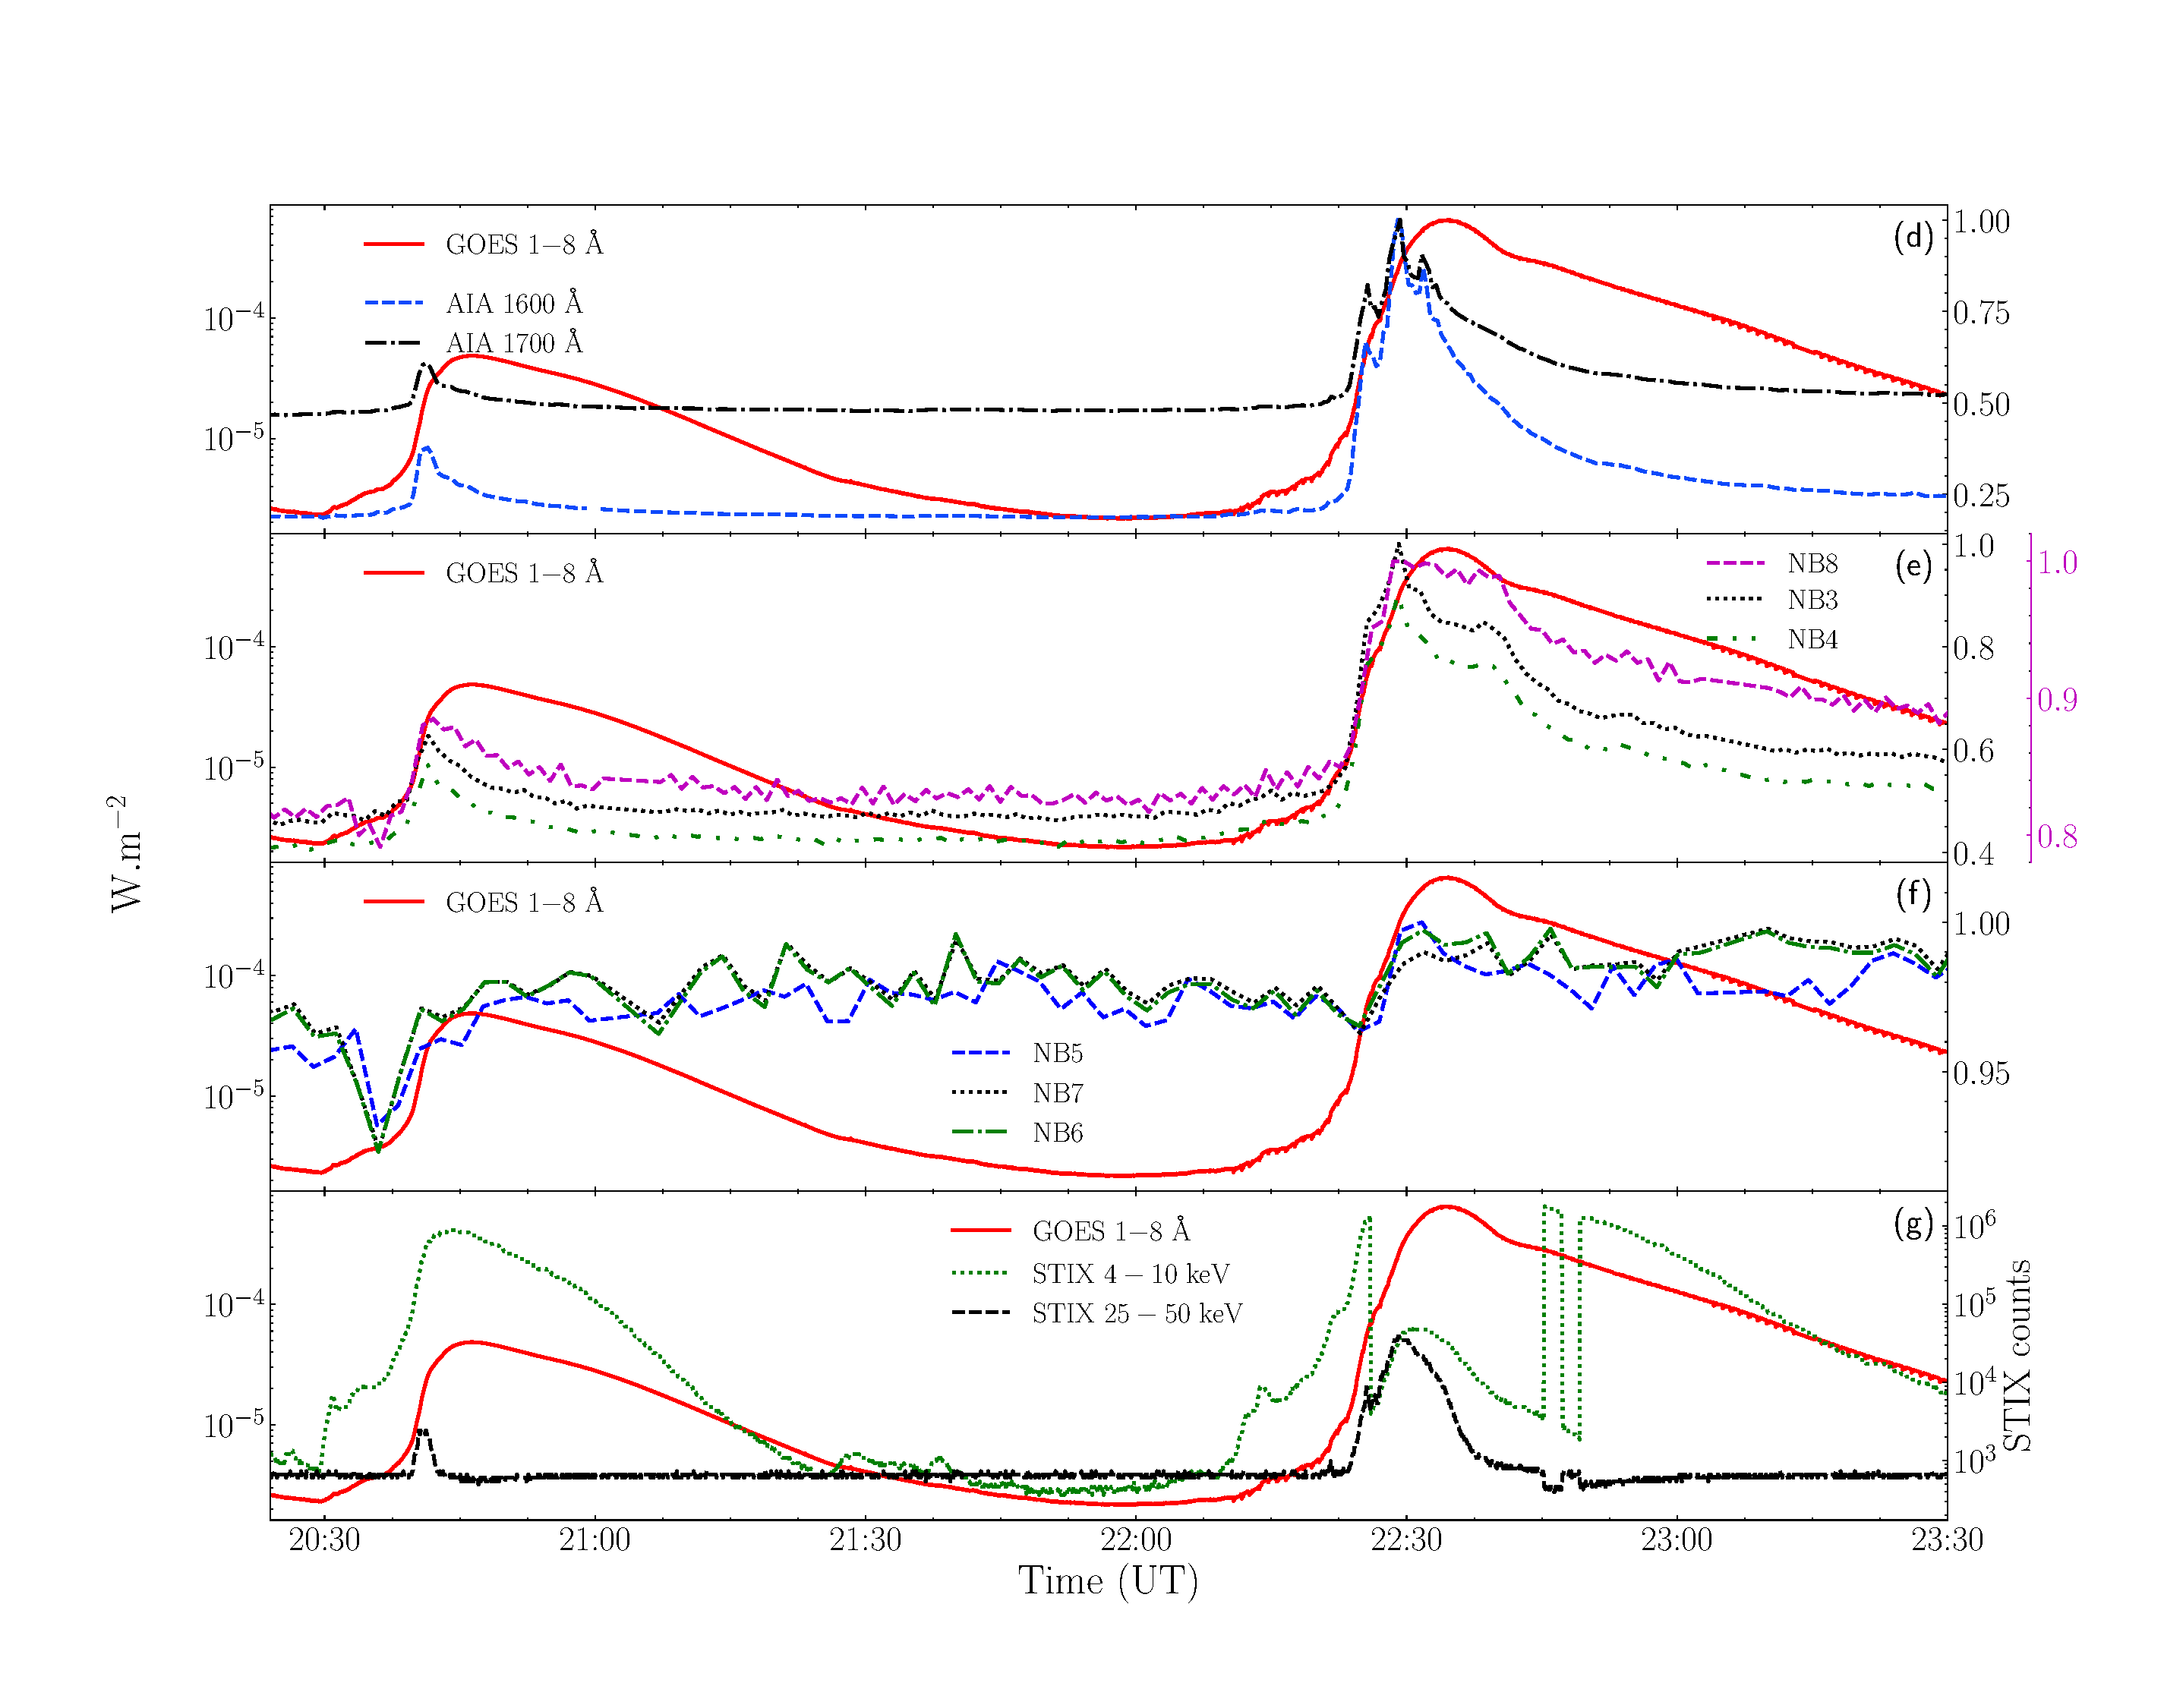
\includegraphics[trim={2.3cm 2.3cm 1.8cm 4.5cm}, clip, width=0.85\linewidth]{fig1_b.pdf}
    \caption{(a) Parts of the full-disk (2k$\times$2k) observation in NB4 (Mg \Romannum{2} h) showing the flaring region and sunspot. The dashed magenta box marks the extent of the \suit~RoI for the flare observation. (b)\suit~RoI observation in NB3 (Mg \Romannum{2} k) during the peak of the flare. The white dashed box shows the region considered for the analysis in this paper. (c) Cutout from the white dashed box marked in (b) of the flare observation in various narrow band filters during their respective peak. (d) {--} (g) \suit~light-curve from the white dashed box in  to various other instruments in various wavelengths (e.g. hard and soft X-ray, extreme ultraviolet etc.)}
    \label{fig:flare_obs}
\end{figure}
%%%%%%%%%%%%%%

%----------------------------------------------------
\begin{table}
\centering
\begin{tabular}{lcr}
\hline
Filter name 	& Central 		    		 & Science\\
		& Wavelength	    	&         Target\\
		& (nm)			    	&          \\
\hline
NB1 		& 214.0                 			&Continuum\\
NB2 		& 276.7 		       			&Continuum\\
NB3 		& 279.6 			   			&Mg~\rm{II}~k\\
NB4 		& 280.3 			   			&Mg~\rm{II}~h\\
NB5 		& 283.2 			   			&Continuum\\
NB6 		& 300.0   			   			&Continuum\\
NB7 		& 388.0   			   			&CN Band\\ 
NB8 		& 396.85 			  				&Ca~\rm{II}~h\\
BB1 		& 200{--}242 		   			&Herzberg Continuum\\
BB2 		& 242{--}300 		   			&Hartley Band\\
BB3 		& 300{--}360 		   			&Huggins Band\\
\hline
\end{tabular}
\caption{Science filters, central wavelength and science target of the 11 science filters for SUIT.} 
\label{sc_comb_fil}
\end{table}
%----------------------------------------------------

%%%%%%%%%%%%%%%%%
\section*{Results}\label{sec:result}
%%%%%%%%%%%%%%%%%

NOAA AR 13590 was visible on the north-east of the Solar disk on February 22, 2024. The AR was around a large sunspot in a cluster of sunspots, accompanied by a complex magnetic field structure. The active region flared multiple times during the same day, including an X1.7 flare that peaked around $\sim$ 06:32 UT, an M4.8 flare that peaked around $\sim$ 20:46 UT and an X6.3 flare that peaked $\sim$ 22:34 UT . \suit~is equipped with an onboard flare detection algorithm. Once the flare detection algorithm flags a flare and localizes the position of the flare on the detector, the program sequence prioritizes reading a fixed smaller Region of Interest (RoI) around the location for fast, higher cadence observation (for further details, please refer to \cite{flare_det}). The X6.3 flare was one of the first flares to be localized by the on-board flare detection algorithm. \suit~did not observe the X1.7 flare because, during that time, the payload was off-pointed to verify the stellar calibration program sequences. The flares were also observed by {\it SDO}/AIA, {\it SO}/STIX. {\it IRIS} observed the eastern edge of the X6.3 flare ribbons in a small [66\arcsec,62\arcsec] field of view (FoV) with a 4 step raster and 15 s raster cadence.

Fig.~\ref{fig:flare_obs}a shows a cutout of the full-disk (2k$\times$2k) observation in NB4 (Mg \Romannum{2} h). The magenta dashed box shows the region observed by the flare mode RoI. Fig.~\ref{fig:flare_obs}b shows the RoI observation in NB3 (Mg \Romannum{2} k) during the peak. The White dashed line shows the region considered for the subsequent analysis in this paper. We plot the observation from the white box marked in Fig.~\ref{fig:flare_obs}b in various \suit~narrow bands during their respective peaks in Fig.~\ref{fig:flare_obs}c. In Fig.~\ref{fig:flare_obs}d {--} g we plot the light-curves arising from the region shown in panel c in comparison to the light-curves in various other wavelengths for two flares in the same region. In Fig.~\ref{fig:flare_obs}d, we plot the AIA 1600 {\AA} (dashed blue line) and AIA 1700 {\AA} (black dot-dashed line), in comparison to the {\it GOES} 1 {--} 8 {\AA} light curve (Solid red line) for both the flares. In Fig.~\ref{fig:flare_obs}e, we show the GOES 1 {--} 8 {\AA} light curve in comparison to the NB3 (Mg \Romannum{2} k 279.6 nm, black dotted), NB4 (Mg \Romannum{2} h 280.3 nm, green dot-dashed) and NB8 (Ca \Romannum{2} h 396.85 nm, magenta dashed) light curves. NB4 light curve is offset from NB3 by -0.1 for better visibility. The NB8 light curve exhibits lower contrast and does not show a sharp peak compared to NB3 and NB4. The other interesting trend is exhibited by the continuum channels NB5, NB6 and NB7 in Fig.~\ref{fig:flare_obs}f, as a conspicuous rise in the continuum intensity is seen after both flares. In Fig.~\ref{fig:flare_obs}g we plot the {\it GOES} 1 {--} 8 {\AA} light curve in comparison to the STIX hard (25 {--} 50 keV, black dashed) and soft (5 {--} 10 keV, green dotted) X-ray light curve. The hard X-ray observation from STIX peaks at a time similar to that of NB3, NB4, and NB8.

The X6.3 flare provides a good example of the response of the local plasma environment to the flare in the Near Ultraviolet (NUV) regime in 200 {--} 400 nm. The flare peaked around $\sim$ 22:34 UT in the {\it GOES} observation. Images from six narrow band (NB) channels of \suit~ are shown in Fig.~\ref{fig:flare_nb3_peak} top panel at around $\sim$ 22:28-22:29 UT. This is at the peak of the NB3 (Mg \Romannum{2} k 279.6 nm) channel, as observed by \suit. The 60\% peak intensity contour of the NB3 intensity is marked with the black line in all figures of Fig.~\ref{fig:flare_nb3_peak} top panel. From the figure, we also see a similar structure in the NB4 (Mg \Romannum{2} h 280.3 nm) and NB8 (Ca \Romannum{2} h 396.9 nm). No similar structure is observed in the other continuum channels of Fig.~\ref{fig:flare_nb3_peak} top panel.

In Fig.~\ref{fig:flare_nb3_peak} bottom panel, we show the flare observations by \suit~ at their respective peaks. Again, we see very similar structures in NB3, NB4, and NB8. NB3 and NB4 peak at almost the same time $\sim$ 22:29 UT. Although NB8 shows a similar structure, the peak intensity of NB8 is observed slightly later around $\sim$ 22:29:41 UT. The peak intensities of the other continuum NB channels are observed progressively later. The NB5 (Red wing of the Mg window) peaks around $\sim$ 22:32:41 UT. Faint signatures of flare brightening are observed in NB5, marked with red arrows in Fig.~\ref{fig:flare_nb3_peak} bottom panel. No such signatures are observed as clearly in NB6 and NB7. Both of these channels peak around $\sim$ 22:28 UT.

%%%%%%%%%
\begin{figure}
    \centering
    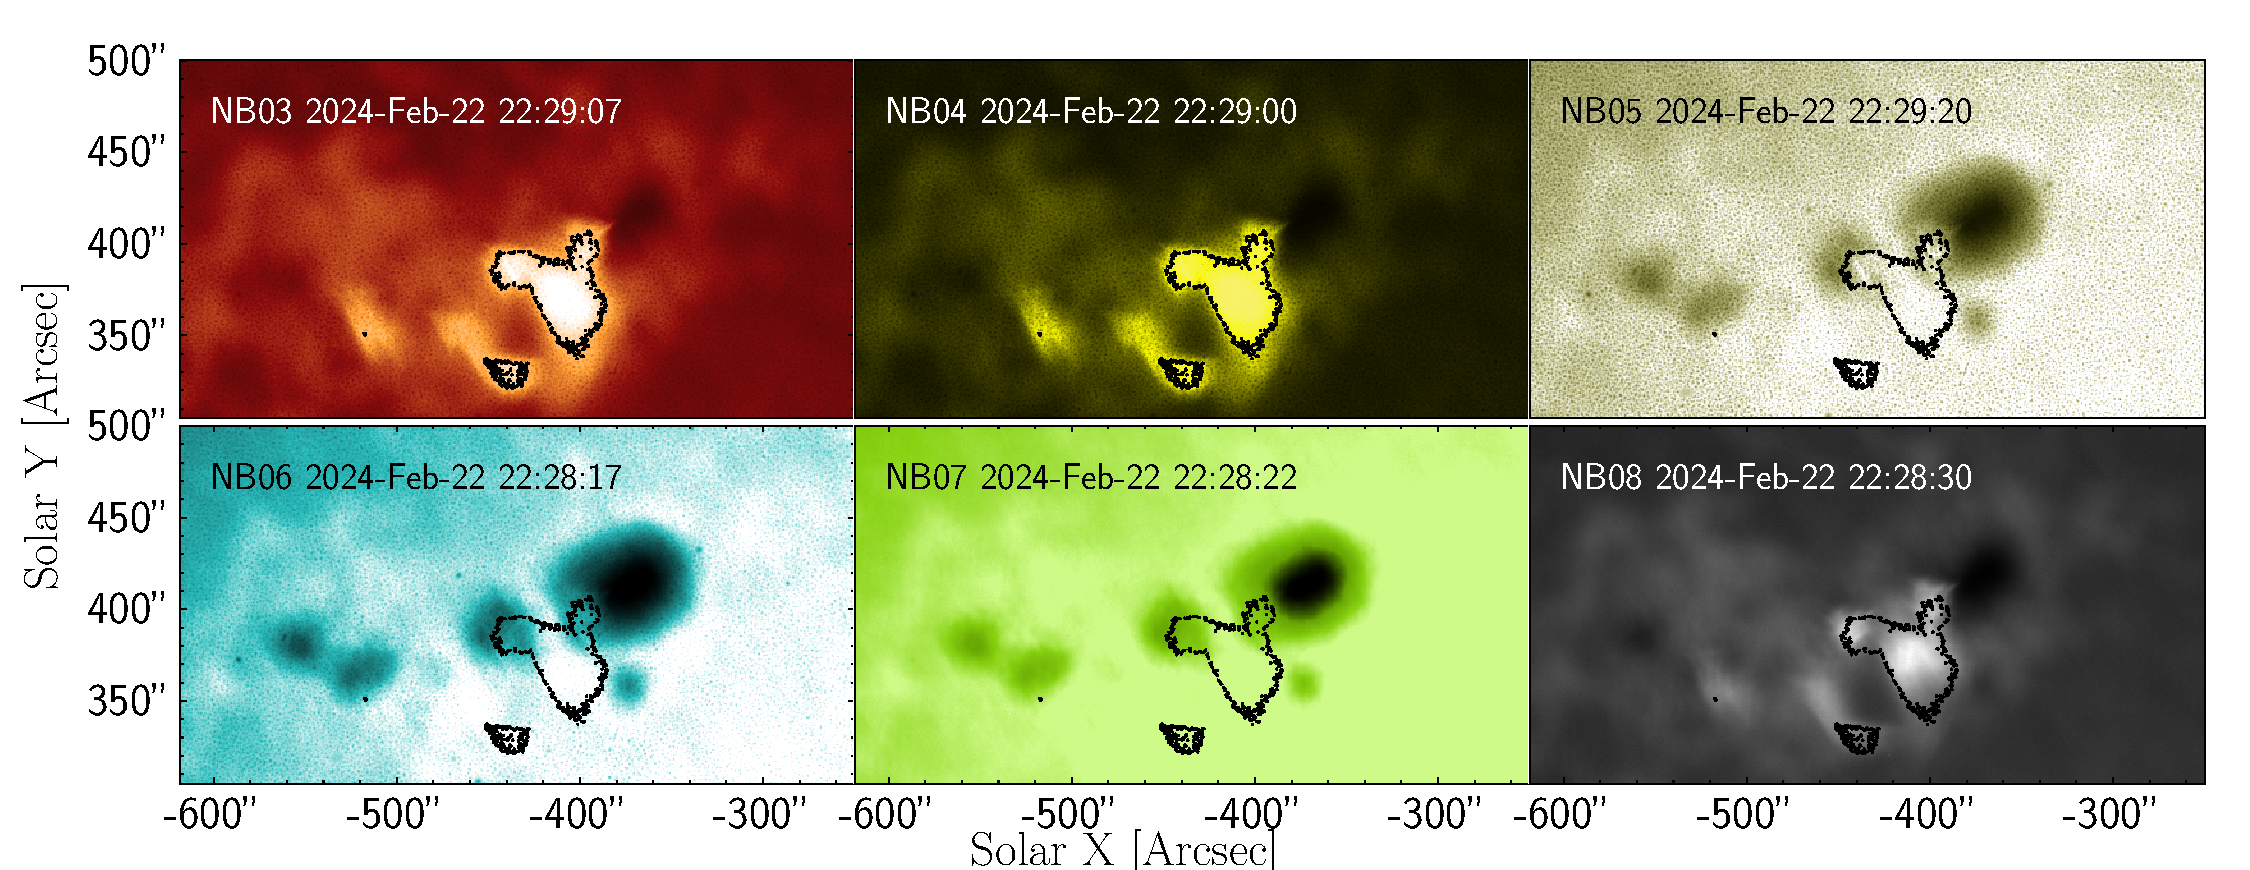
\includegraphics[trim={0cm 0.65cm 0cm 0cm},clip,width=0.7\textwidth]{suit_roi_nb3_peak.pdf} \\
    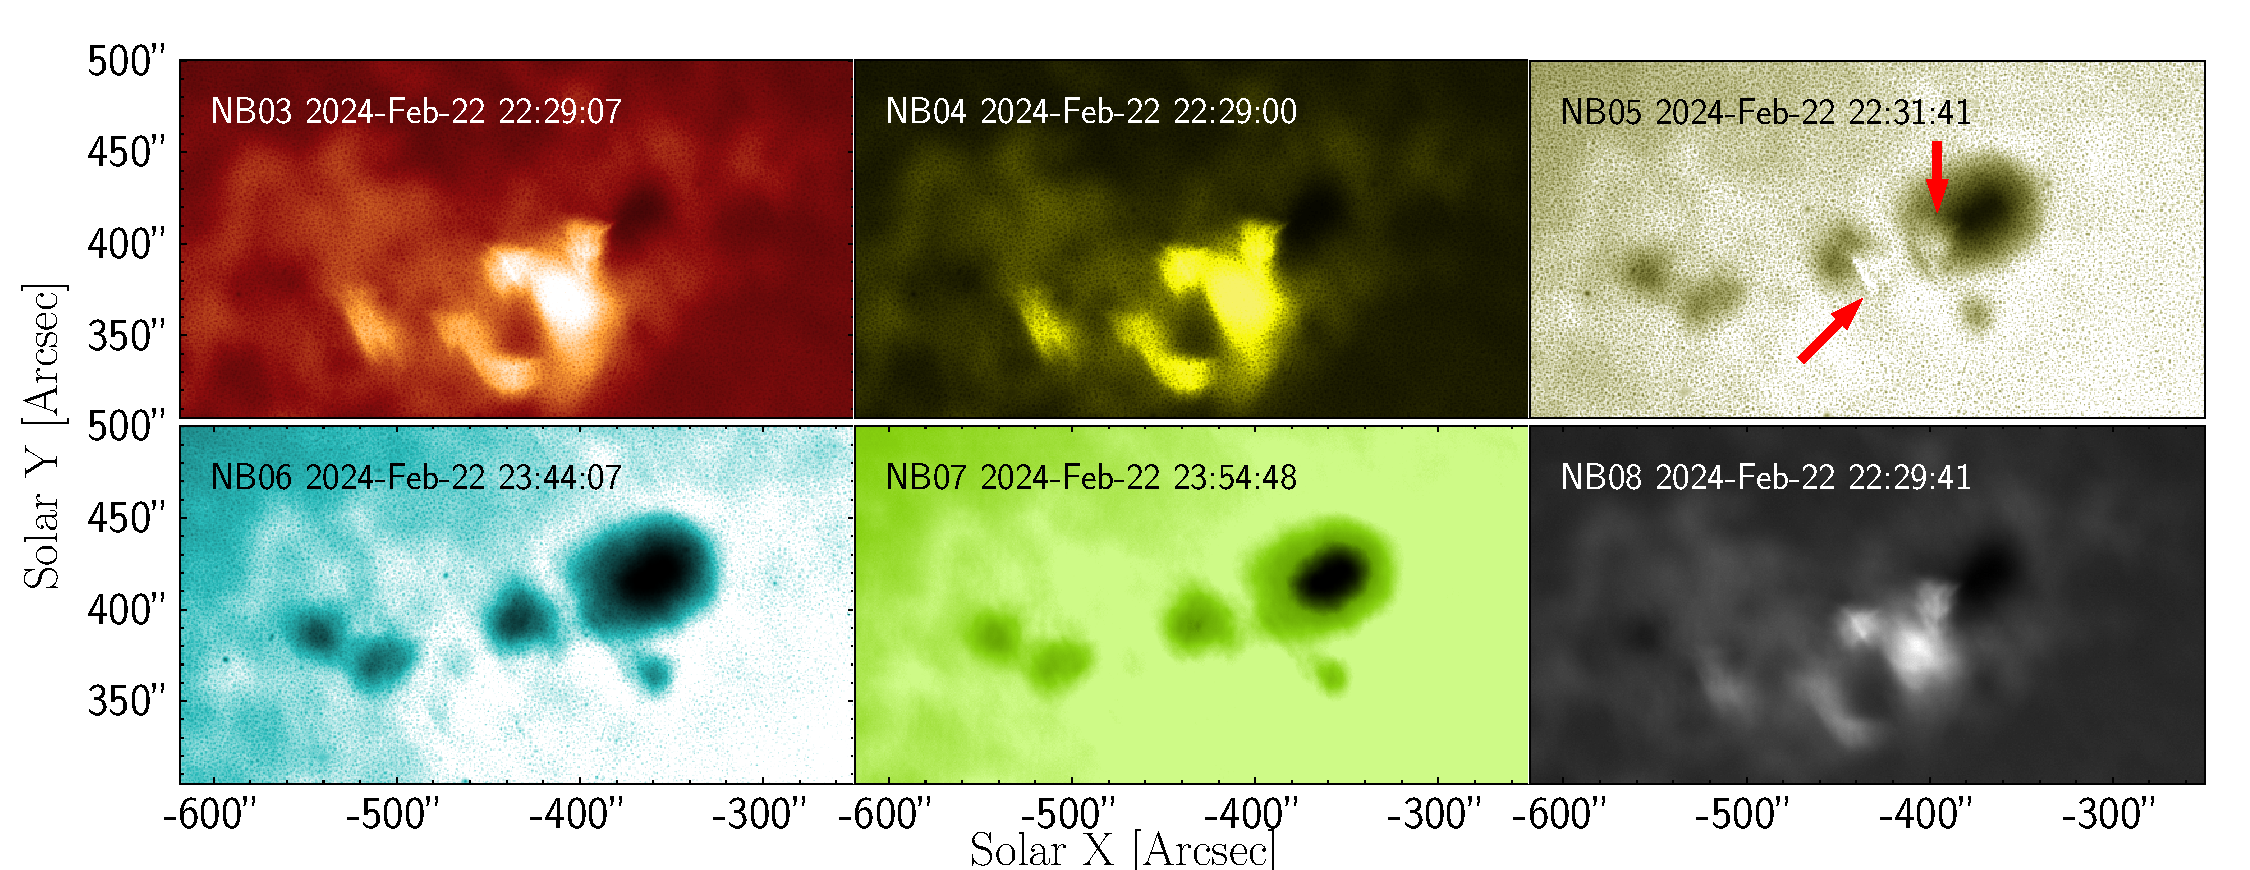
\includegraphics[width=0.7\textwidth]{suit_roi_all_peak.pdf}
    \caption{\suit~observations of the flare from various NB filters. Top panel: during NB3 peak. Bottom panel: During the peak of individual bands.}
    \label{fig:flare_nb3_peak}
\end{figure}
%%%%%%%%%

In Fig.~\ref{fig:flare_lc_suit}, we plot the light curve of the event to compare the observations across various bands. The AIA and \suit~ light curves in Fig.~\ref{fig:flare_lc_suit} are calculated by adding the counts within the region of 60\% peak intensity contour of NB3 (shown in Fig.~\ref{fig:flare_nb3_peak} top panel), after co-aligning and registering the AIA and \suit~observations and normalizing them to the peak intensity. In Fig.~\ref{fig:flare_lc_suit}.a, we show the GOES 1 {--} 8 {\AA} light curve in comparison to AIA 1600 {\AA} and AIA 1700 {\AA}. The AIA 1600 and 1700 {\AA} light curve peaks around $\sim$ 5 minutes earlier than the {\it GOES} peak. 

In Fig.~\ref{fig:flare_lc_suit}.b, we show the GOES 1 {--} 8 {\AA} light curve in comparison to the NB3, NB4 and NB8 light curves. All the NB light curves behave remarkably similarly. The vertical dotted black line across all the panels in Fig.~\ref{fig:flare_lc_suit} denotes the peak intensity in NB3. NB3, NB4, and NB8 peaks around $\sim$ 22:29 UT, which is very similar to AIA 1600 {\AA} and 1700 {\AA}. We also plot the {\it GONG}-H$\alpha$ light curve from the \suit~contour region. The {\it GONG} light curve also peaks at around $\sim$ 22:29 UT. Both NB8 and {\it GONG}-H$\alpha$ shows less contrast variation in the light curve than NB3 and NB4.

We show the GOES 1 {--} 8 {\AA} light curve in comparison to the NB5 (Red wing of the Mg lines, blue dashed), NB6 and NB7 continuum channels in Fig.~\ref{fig:flare_lc_suit}.c. NB5 shows signs of flare response, although much weaker than NB3, NB4 and NB8. NB5 peaks around $\sim$ 22:31 UT, about $\sim$ 3 minutes later than NB3. Similar traits were observed from the images also, as pointed out in Fig.~\ref{fig:flare_nb3_peak} bottom panel and the accompanying discussions. More interestingly, NB6 and NB7 do not show the hallmark sign of a flare light curve, i.e. gradual increase and decrease in the intensity. These bands exhibit a slow but steady rise in intensity after the flare. Finally, in Fig.~\ref{fig:flare_lc_suit}.d, we show the {\it GOES} 1 {--} 8 {\AA} light curve in comparison to the STIX hard and soft X-ray light curve. The hard X-ray peaks around a similar time around $\sim$ 22:29 UT, similar to NB3, NB4 and AIA 1600 and 1700 {\AA}.

%%%%%%%%%
\begin{figure*}
    \centering
    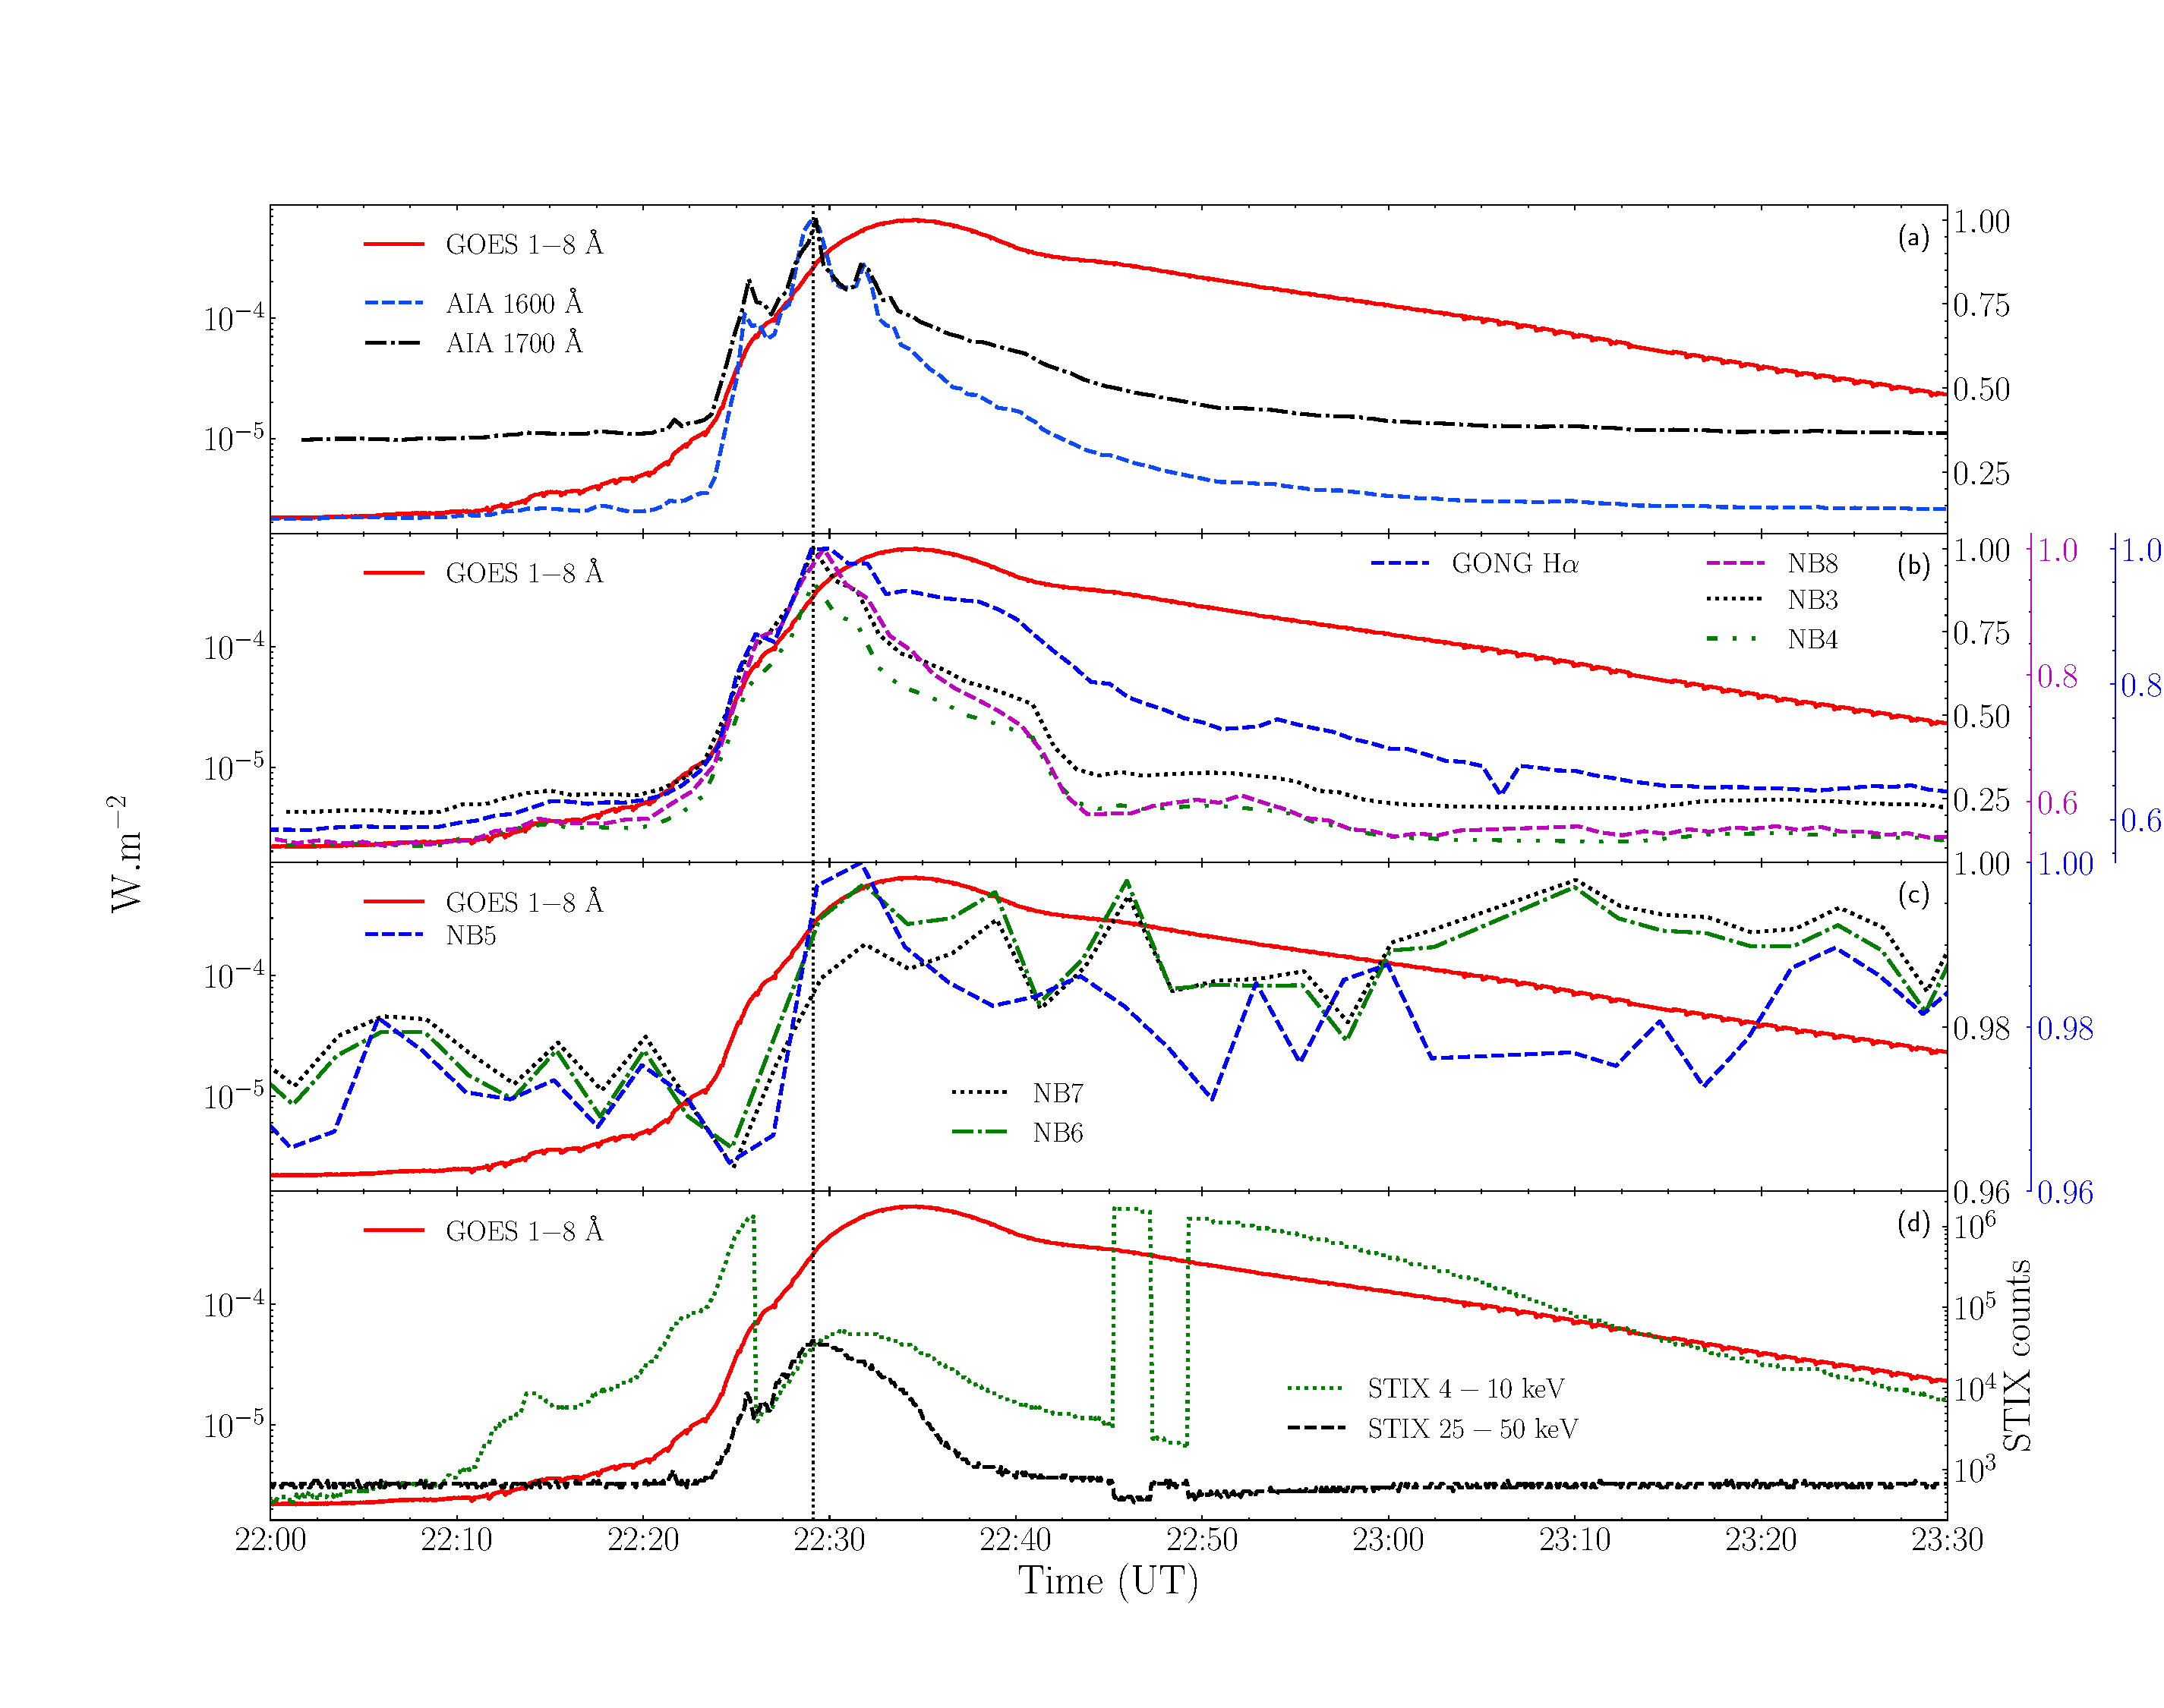
\includegraphics[width=0.9\textwidth,trim={2.3cm 2.5cm 0cm 4.5cm},clip]{lc_suit_contour.pdf}
    \caption{Light curves from the pixels within intensity contour picked from \suit~and co-aligned AIA observations. The NB4 light curve in the second panel is offset by -0.1 from NB3 for better visibility. The vertical dotted dark line marks the flare's peak in NB3 observation.}
    \label{fig:flare_lc_suit}
\end{figure*}
%%%%%%%%%

%%%%%%% ############# %%%%%%%
%\subsection*{XSM-spectra}\label{sec:xsm}
%%%%%%% ############# %%%%%%%

The Solar X-ray monitor on {\it Chandrayan-2}\citep[{\it Chandrayan-2}/XSM,][]{xsm} provides sun as a star soft X-ray spectra in 1{--}15 keV with 1s cadence and significantly better spectral resolution (180 eV at 5.9 keV) compared to STIX (1 keV at 5.9 keV). The high spectral and temporal resolution allows us to measure the change in elemental abundances over the duration of the flares. XSM observed both flares with coverage in both impulsive and decay phase. The existing studies with XSM has successfully studies the thermal and elemental abundance evolution of various flares \citep{mondal21,kkepa23,nama23}.

Both the M and X-class flares were observed by XSM. The XSM 1{--}8 {\AA} light curves are plotted in Fig.~\ref{fig:xsm-obs} top panel. The red shaded region marks the time window where the Be filter was inserted to prevent saturation. There are periodic gaps in the data due to periodic lunar occultation. We show the spectra obtained by XSM in Fig.~\ref{fig:xsm-obs} bottom panel, during various phases of the flare. The violet spectra at 22:33 UT is near the flare peak, and shows a sharp decrease below 3 keV due to the insertion of the Be filter to avoid saturation. Various Mg, Al, S and Si lines are visible in the pre-flare spectra. In stark contrast during impulsive and peak of the flare we see strong signatures of Ca, Ar and Fe. Due to the uncertainty of the spectra during the Be window observation in $<~3~\mathrm{keV}$ regime, we fit the spectra beyond 3 keV throughput this analysis. We fit the spectra with the XSPEC model `{\it chisoth}', which uses a wide range of pre-calculated spectra to fit the observed spectra (For more details please refer to the appendix of \cite{mondal21}).

%%%%%%%%
\begin{figure}
    \centering
    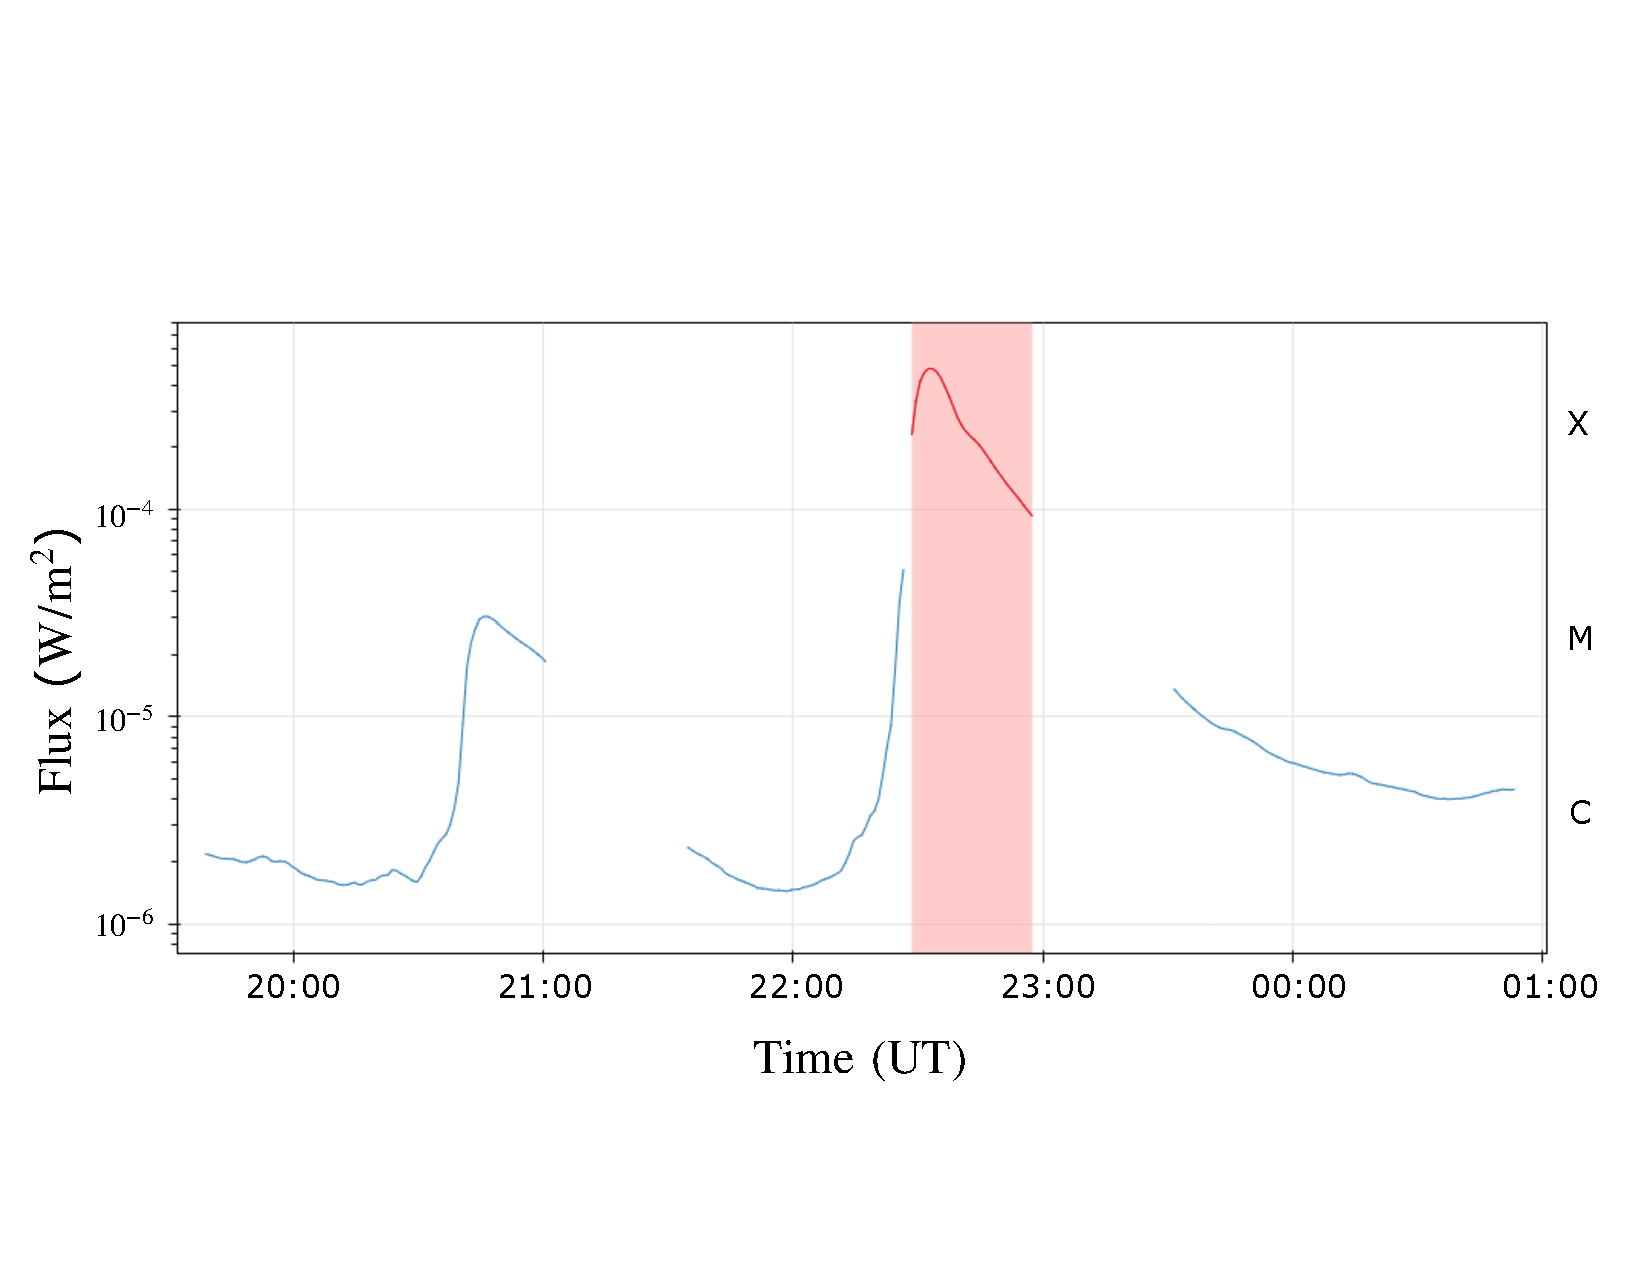
\includegraphics[trim={0.5cm 3.3cm 0.8cm 4cm}, clip, width=0.61\textwidth]{xsm_lc.pdf} \\
    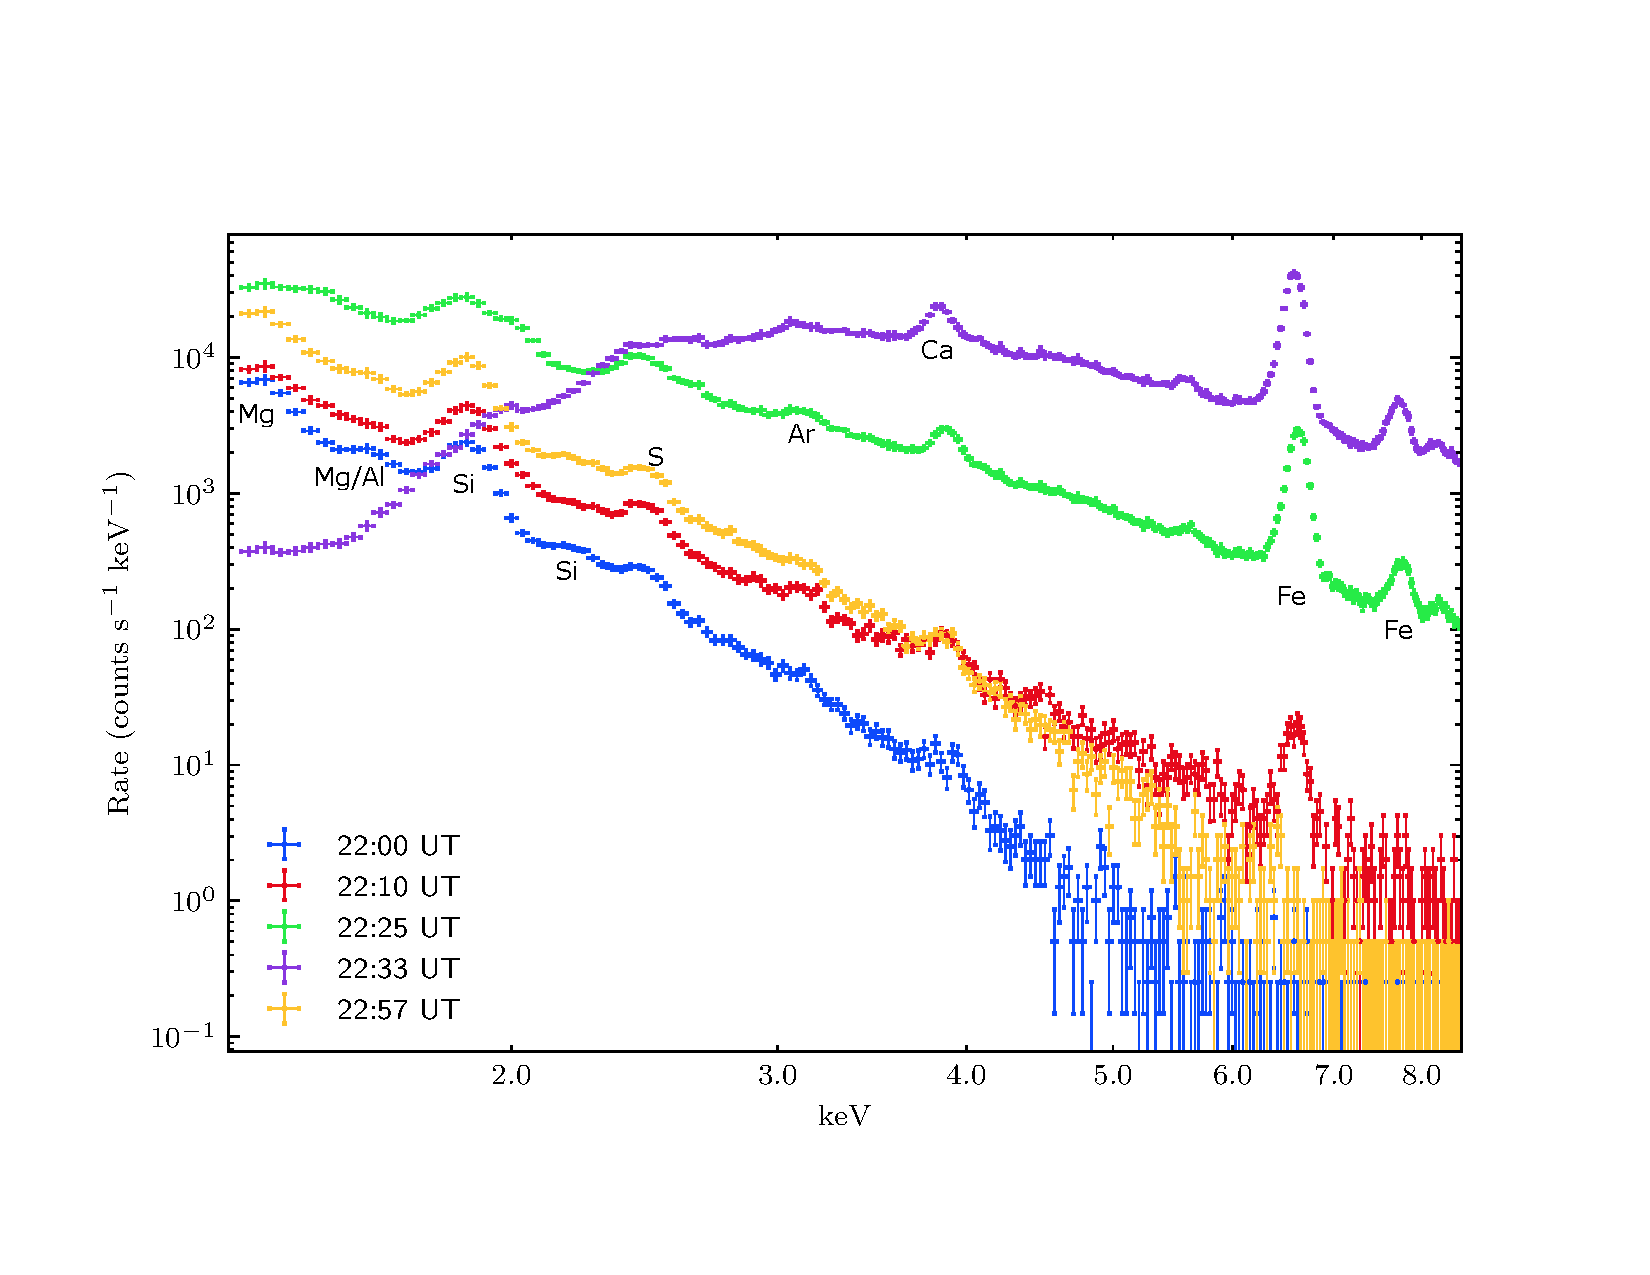
\includegraphics[trim={1.8cm 2.5cm 3cm 3cm},clip,width=0.6\textwidth]{xsm_spec.pdf}
    \caption{Top panel: XSM observation of the two flares. The red shaded region marks the window when the Be filter was inserted. Bottom panel: X-ray spectra during various phases of the flare. The violet spectra is during the soft X-ray peak of the flare and shows a sharp decrease in the intensity below 3 keV. This is due to the insertion of Be filter to avoid saturation.}
    \label{fig:xsm-obs}
\end{figure}
%%%%%%%%

One of the key observations we make is a presence of systematic residual around the Fe complex around $\sim$ 6.5 keV (please refer to the top panel of Fig.~\ref{fig:xsm_fit} top panel, where there is an excess visible in the blue side of the Fe line complex at $\sim$ 6.7 keV). \cite{mithun22} could not explain this systematic excess with multithermal DEM distributions. {\bf Is it possible we are missing some line in ``chisoth"?} One of the possible explanation of this excess flux is Fe fluorescence emission. There have been observations of Fe line fluorescence at 6.4 keV (Fe K$\alpha$) and 7.06 keV (Fe K$\beta$) \citep{neupert67,doscheck71,bai79,tanaka84,parmar84,phillips12} using high-resolution X-ray spectra from Bent Crystal Spectrometer on-board Solar Maximum Mission \citep[Bent/{\it SMM},][]{bent,smm} and Yokoh \citep{yokoh} mission. Previous studies have suggested that this emission arises from the excitation of low ionization state Fe in the Photosphere either via the X-ray from the flaring plasma \citep{bai79} or directly from the non-thermal electron beam \citep{phillips73}. The Fe K$\alpha$ fluorescence is usually dependent on the position on the solar disk \citep{parmar84}. The emergent Fe K$\alpha$ emission suffers significant absorption and scattering along the line of sight, which increases with increasing heliocentric angle, resulting in a decrease in the observed intensity. For our event, the flaring region is near the disk center making the Fe K$\alpha$ fluorescence a valid candidate for explaining the excess.

We add a Gaussian line component to our fit at 6.4 keV to explore the possibility of the excess flux arising from Fe K$\alpha$ fluorescence. We find that this fits the observed spectra better than previous instances, as demonstrated in Fig.~\ref{fig:xsm_fit} bottom panel. The K$\alpha$ emission would arise from the X-ray emission from the flaring regions having energies $>$ 7.12 keV, the K edge of Fe, exciting the Fe atoms in the Photosphere. We show the intensity of the fitted Fe 6.4 keV component excess (blue solid line), in comparison to the fitted flux in 7.12 {--} 8.5 keV (green dot-dashed line) in Fig.~\ref{fig:fe_excess} top panel. For reference, {\it GOES} 1{--}8 {\AA} soft X-ray flux (red dotted line) and STIX 25 {--} 50 keV Hard X-ray flux (black dashed line) are overplotted. STIX Hard X-ray is a fair representative of the non-thermal electron flux deposited into the foot points. In the middle panel, the light curve of fitted Fe 6.4 keV excess Gaussian component is plotted (blue solid line) with the light-curve from the bright kernels marked with the two boxes in Fig.~\ref{fig:fe_excess} top panel NB5 observation. In Fig.~\ref{fig:fe_excess} bottom panel the light-curve of the 6.4 keV excess component (blue solid line) is plotted with the light-curve from the bright kernels marked with the two boxes in Fig.~\ref{fig:fe_excess} top panel NB2 observation. In all panels, the peak time of the Fe excess (blue solid line), STIX hard X-ray (black dashed line) and NB5 brightness from box 1 (dotted magenta line) are marked with vertical lines.

%%%%%%%%%%
\begin{figure*}
\centering
    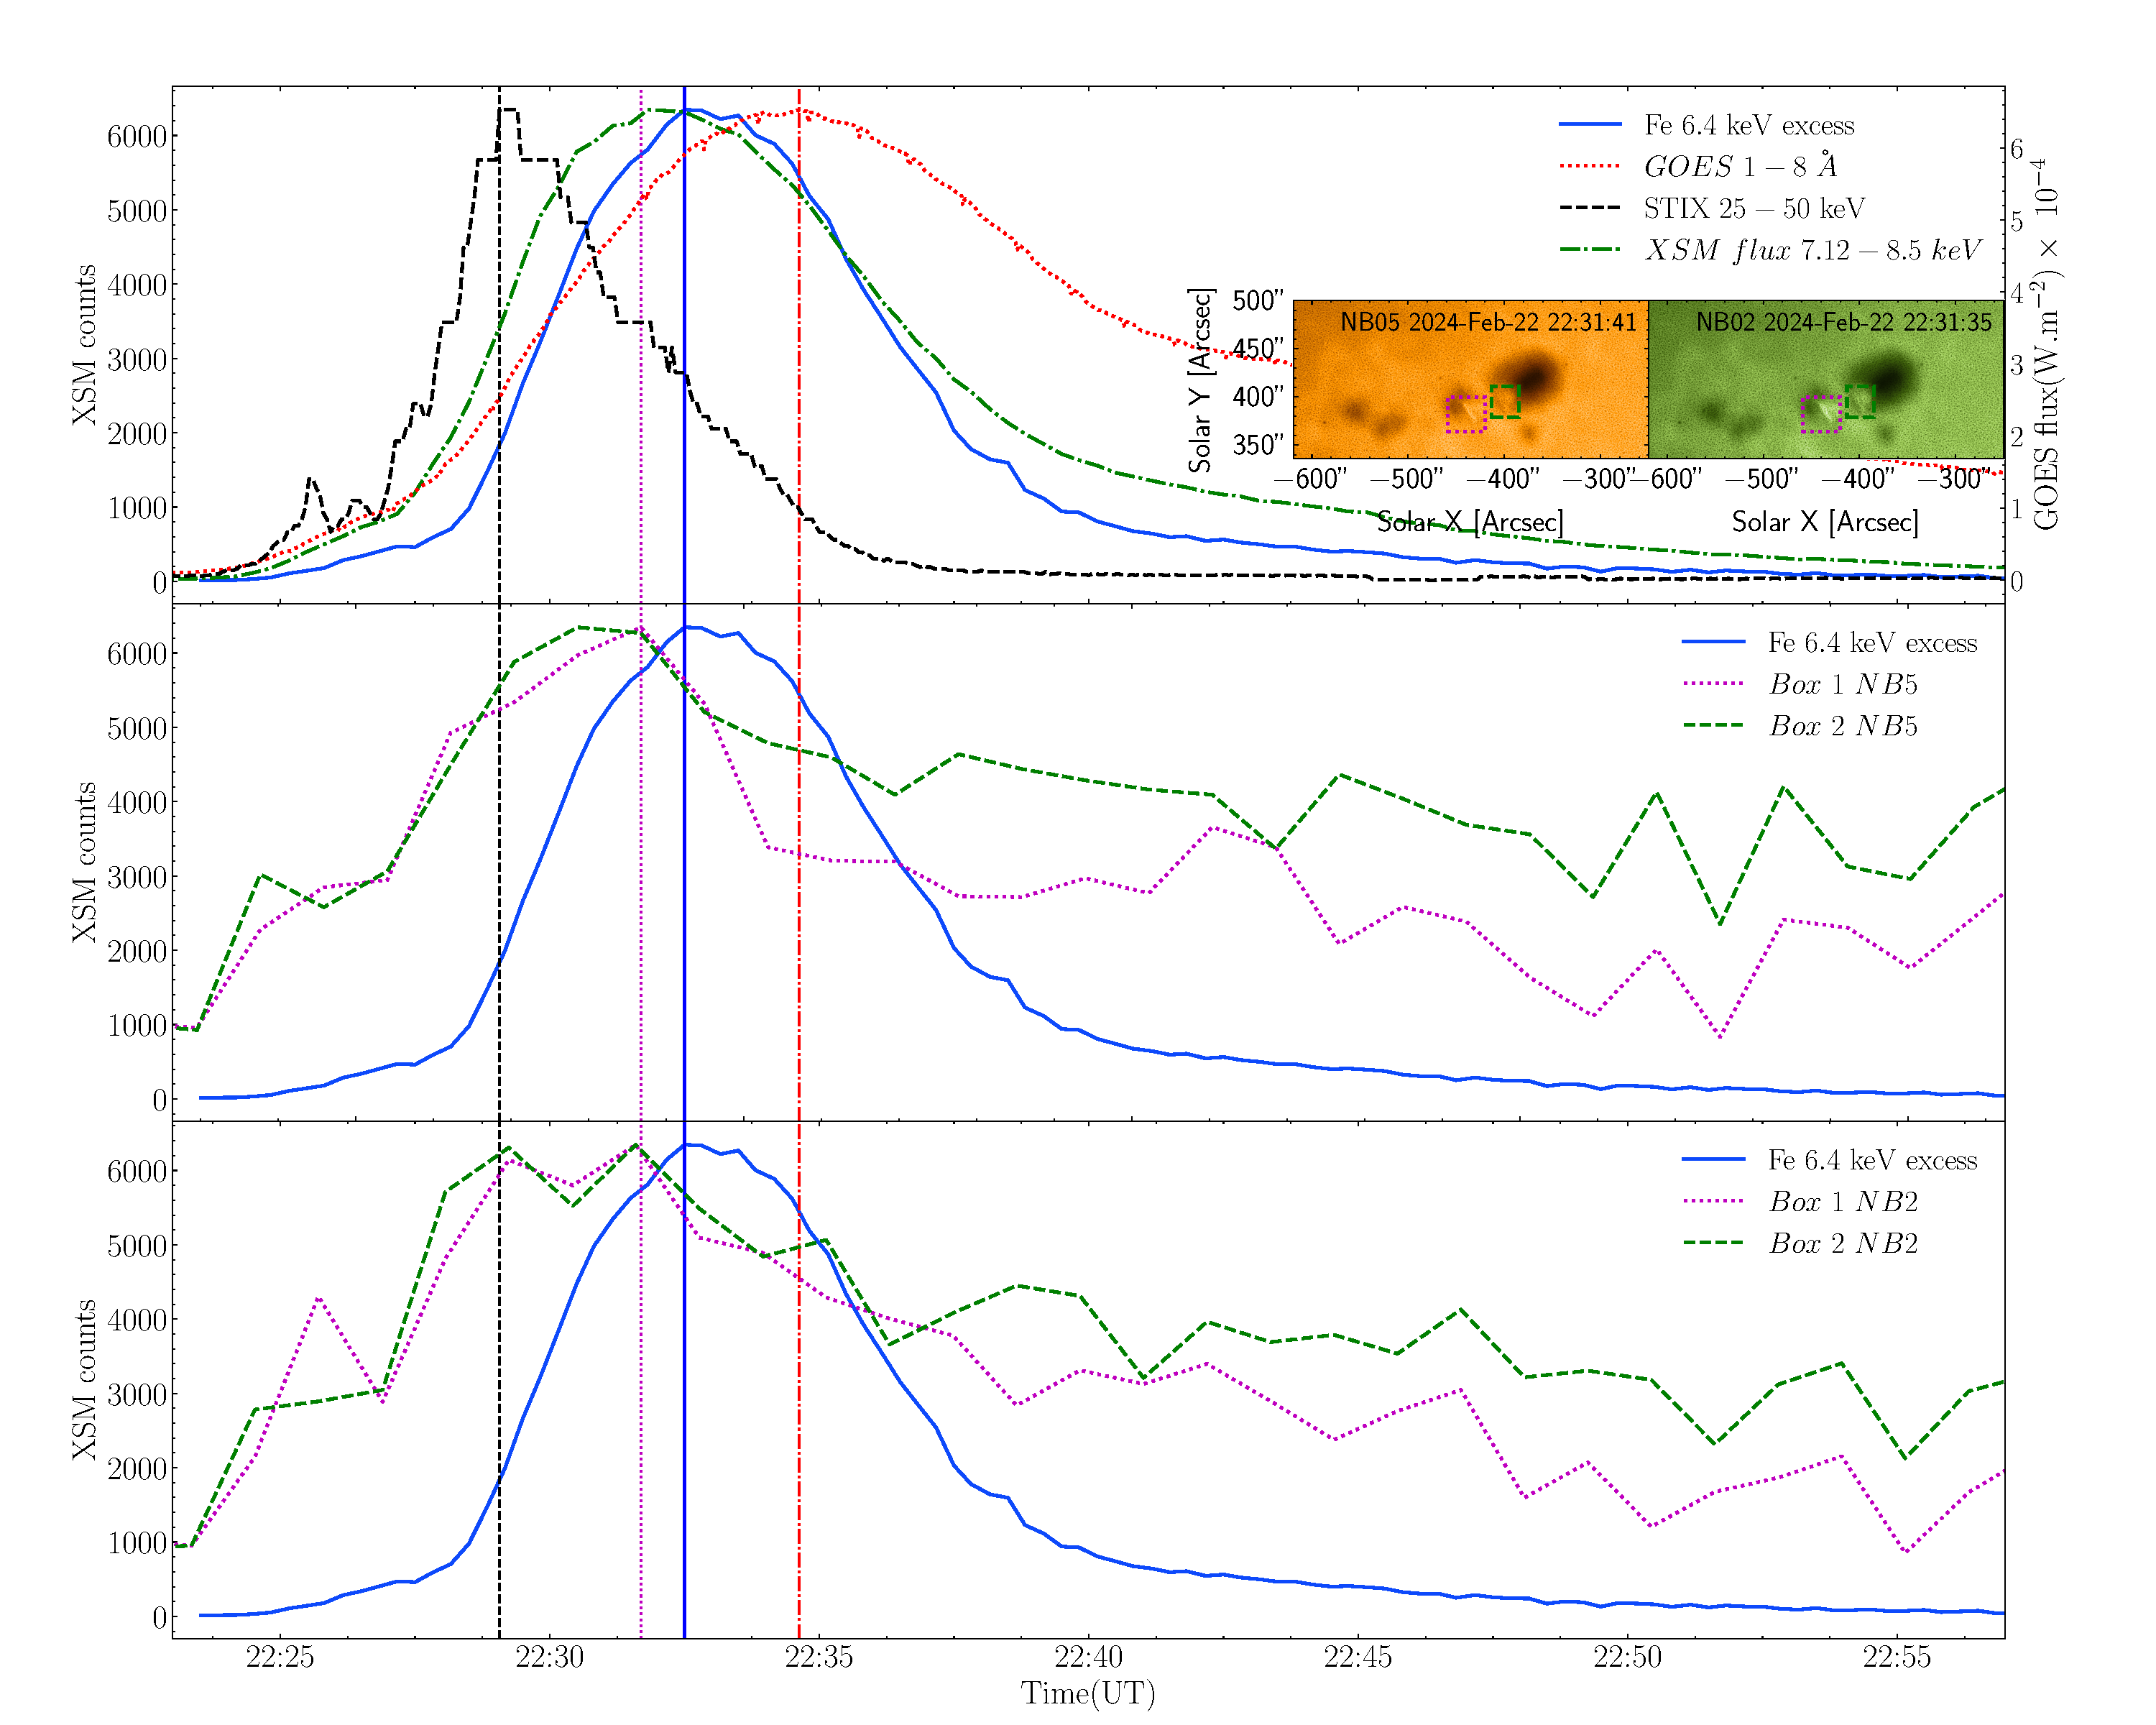
\includegraphics[trim={1.7cm 0.5cm 2.3cm 1.9cm}, clip, width=0.9\textwidth]{fe_excess_4.pdf}
    \caption{Fe excess emission from 6.4 keV(blue solid) in comparison to STIX 25-50 keV(black dashed), GOES 1 {--} 8 $\AA$ (dotted red) and XSM 7.12 {--} 8.5 keV (green dot-dashed) light curve.}
    \label{fig:fe_excess}
\end{figure*}
%%%%%%%%%%

%%%%%%% ############# %%%%%%%
\section*{Discussion}\label{sec:dis}
%%%%%%% ############# %%%%%%%

This paper reports the \suit~narrowband imaging of the first localized flare by the onboard flare detection algorithm. We report the observation in NB3 (Mg \Romannum{2} k 279.6 nm), NB4 (Mg \Romannum{2} h 280.3 nm), NB8 (Ca \Romannum{2} h 396.9 nm) and the continuum channels NB5 (Red wing of Mg \Romannum{2}), NB6 and NB7. For both the flares, the NB3, NB4 and NB8 peak around the same time as AIA 1600 and 1700 {\AA}. For the X6.3 flare, NB3, NB4 behave very similarly to NB8 within the NB3 intensity contour (see Fig.~\ref{fig:flare_lc_suit}.b). But the NB8 peak over the whole active region is much broader compared to the NB3 and NB4 light curves (see Fig.~\ref{fig:flare_obs}). This implies that NB8 behaves differently in other parts of the active region.

The NB5 observes the continuum that is usually attributed as the Balmer continuum. There have been previous studies where Photospheric metal lines went into emission and affected the Balmer continuum \citep{heinzel14,kleint17}. The dominant contribution would still be the Balmer continuum. \cite{reetika21} attributed the brightening in the SJI 2832 {\AA} continuum for a mini flare to direct signature of electron beams. \cite{kowalski19} showed for one event, that the SJI 2832 {\AA} continuum enhancement and several Phototspheric absorption lines going into emission can be attributed to significant Photospheric heating. The entire 2832 {\AA} window of IRIS had several Fe \Romannum{2} and Cr \Romannum{2} lines which are usually observed as absorption lines, in emission. Curiously enough, this observation was also made in a bright umbral flare kernel, similar to the current event. As there was no {\it IRIS} scan of the umbral brightening visible in NB5, unfortunately, we can not comment on the spectral nature of the bright kernel.

We see an excess around the 6.5 keV Fe complex from the XSM observations which can be fitted with a single Gaussian. From Fig.~\ref{fig:fe_excess}, the Fe excess light curve (blue solid line) behaves very similar to the soft X-ray flux beyond the Fe K edge at 7.12 keV (green dot-dashed line). The excess also shows no correlation with the STIX 25 {--} 50 keV hard X-ray flux (black dashed line), illustrating no significant contribution from the non-thermal electron flux. This suggests that the excess flux seen around 6.4 keV Fe complex arises from the Fe fluorescence from the flaring X-ray. If we assume the penumbral brightening observed in this flare to be similar as observed by \cite{kowalski19}, the bright kernels observed in NB5 mainly arises from a plethora of Fe \Romannum{2} lines. The flaring X-ray beyond Fe K edge (7.12 keV) photoionizes the Fe in the Photosphere, giving rise to both Fe \Romannum{2} lines in the red wing of Mg \Romannum{2}, along with the observed Fe fluorescence by XSM. 

We see a similar brightening in NB2, the blue wing of the Mg window. The light curve of the brightening of the blue wing of Mg is shown in Fig.~\ref{fig:fe_excess} third panel. The light curve shows peak at both hard X-ray peak and later on closer to Fe excess component peak. This possibly shows both Photospheric and Chromospheric components from the NB2. Further investigation and modelling is required to comment on the local plasma parameters that would produce the bright kernels observed in both NB5 and NB2, with the relative timing within themselves and also in comparison to the various energies in X-ray.

The other interesting observation is the rise in the continuum intensity, specifically in NB6 and NB7 as the flares happen. We can see a steady rise in the continuum intensity after the M and X class flare (see Fig.~\ref{fig:flare_obs}). For the X6.3 flare, we do see some signature of the flare in NB5, although it peaks about $\sim$ 5 minutes later compared to NB3 and NB4. The photospheric nature of the NB5 continuum explains the 5-minute delay of the peak from NB3. We see the flare peak in sequential order of formation height NB3 and NB4 (Mg \Romannum{2}, 22:29 UT) and NB8 (Ca \Romannum{2}) $\Longrightarrow$ NB5 (Photospheric continuum, 22:32:41 UT). We are observing the increase in continuum intensity from 283.2 nm to 388 nm. The consistent increase in continuum intensity is happening across the Balmer jump ($\lambda$~=~364.5 nm).

%%%%%%%%%%%%%%%%%%%%%%%%%%%%%%%%%%%%%
\section*{Methods}\label{sec:met}
%%%%%%%%%%%%%%%%%%%%%%%%%%%%%%%%%%%%%

\subsection*{XSM Spectra Fitting}

The observed soft X-ray spectra from the flaring plasma can be modelled by an isothermal plasma characterized by various parameters {\it e.g.} temperature, emission measure and abundance of various elements. As alluded earlier, we use the `{\it chisoth}' model \citep{mondal21} to fit the observed spectra from XSM. The `{\it chisoth}' model uses CHIANTI atomic database \cite{chianti} to calculate spectra for individual elements over a large temperature grid and stores as tables. The model includes elements from H (Z=1) to Zn (Z=30). The spectra of individual elements are calculated over a wide temperature range (0.3 {--} 50 MK). These modelled spectra of various elemental abundance over a wide temperature range are loaded in XSPEC and added with varying weights to fit the observed spectra. The Total model spectrum is given by  $$I_{mod}(T)~=~EM\sum_{X}I_{X}(T)N_{X}$$`EM' is the volume emission measure, $N_{X}$ is the abundance of element X relative to H and $I_{X}(T)$ is the modelled spectrum of element X at temperature T. The fit is done in a recursive process by minimizing the chi-squared between the observed and modelled spectra.

We initially used an isothermal model to fit the spectra. As alluded earlier in \S\ref{sec:result}, we see an excess around 6.4 keV (see Fig.~\ref{fig:flare_obs} top panel). We added a Gaussian component to the `{\it chisoth}' model to get better fit (see Fig.~\ref{fig:flare_obs} bottom panel).

%%%%%%%%%%
\begin{figure}
    \centering
    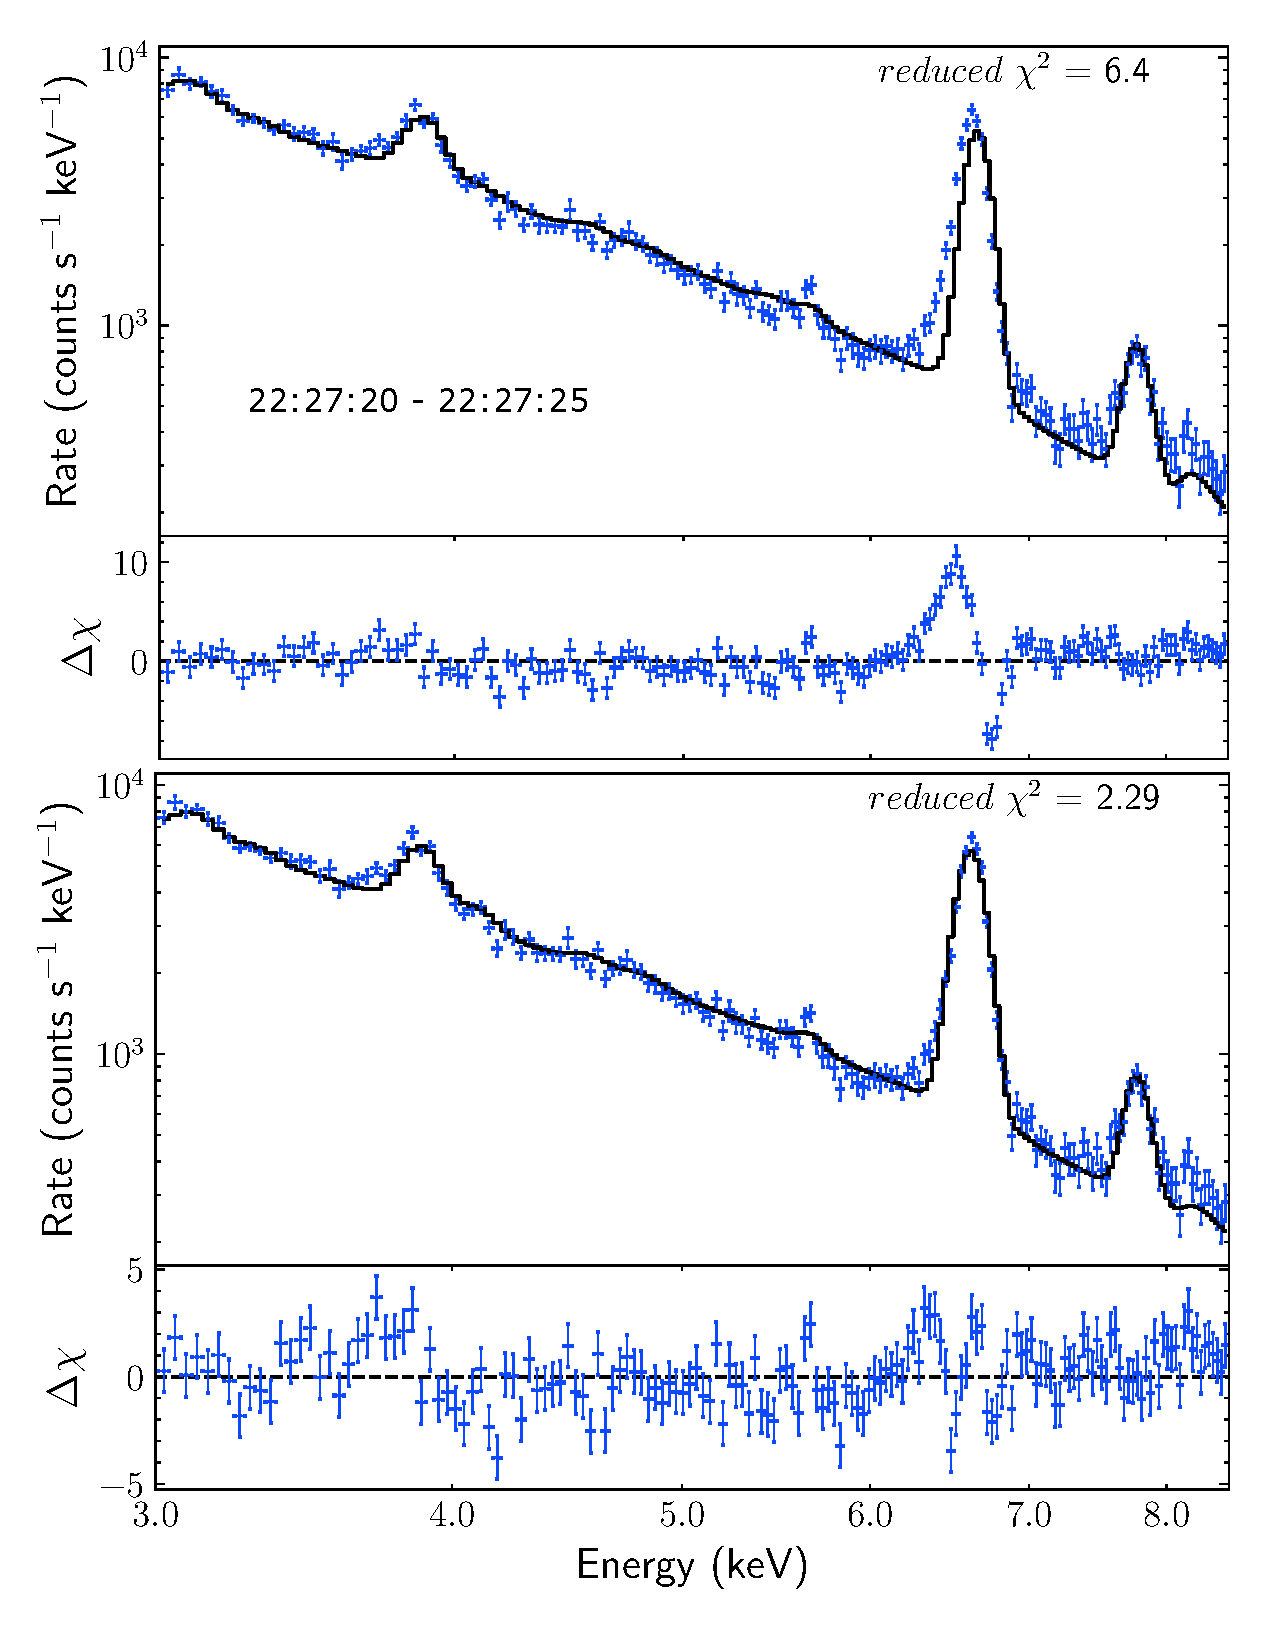
\includegraphics[trim={0.5cm 1cm 0.5cm 0.7cm}, clip, width=0.6\textwidth]{xsm_fit.pdf}
    \caption{XSM spectra in 3 {--} 8.5 keV binned between 22:27:20 {--} 22:27:25 UT. Top panel shows the fit with ``chisoth" model. Bottom panel shows the same spectra fitted with ``chisoth+gaussian" model.}
    \label{fig:xsm_fit}
\end{figure}
%%%%%%%%%%

\section*{Data Availability}
The AIA data used in this study are publicly available at Joint Science Operations Center (JSOC, \href{http://jsoc.stanford.edu/}{http://jsoc.stanford.edu/}). The STIX data is openly available in ESA Solar Orbiter Archive (\href{https://soar.esac.esa.int/soar/}{https://soar.esac.esa.int/soar/}). The XSM data is publicly available in ISRO Science Data Archive (ISDA, \href{https://pradan.issdc.gov.in/ch2/}{https://pradan.issdc.gov.in/ch2/}). The GONG data products are publicly available at GONG Data Archive (\href{https://gong2.nso.edu/archive/patch.pl}{https://gong2.nso.edu/archive/patch.pl}). {\bf What about \suit~data availability?}

\backmatter

\bmhead{Acknowledgments}
IRIS is a NASA small explorer mission developed and operated by LMSAL with mission operations executed at NASA Ames Research Center and major contributions to downlink communications funded by ESA and the Norwegian Space Centre. {\bf Do we have an acknowledgement like this for overall Aditya-L1 mission?}The AIA data used here are courtesy of SDO (NASA) and the AIA consortium. Solar Orbiter is a space mission of international collaboration between ESA and NASA, operated by ESA. The STIX instrument is an international collaboration between Switzerland, Poland, France, Czech Republic, Germany, Austria, Ireland, and Italy. CHIANTI is a collaborative project involving George Mason University, the University of Michigan (USA), University of Cambridge (UK) and NASA Goddard Space Flight Center (USA). We acknowledge the use of data from the Solar X-ray Monitor (XSM) on board the Chandrayaan-2 mission of the Indian Space Research Organisation (ISRO), archived at the Indian Space Science Data Centre (ISSDC). XSM was developed by Physical Research Laboratory (PRL) with support from various ISRO centers. This research used version 4.1.5 \citep{sunpy_ver} of the SunPy open-source software package \citep{sunpy20} and PYTHON packages NumPy \citep{numpy}, Matplotlib \citep{matpltolib}, SciPy \citep{scipy} and SciencePlots \citep{SciencePlots}.

\begin{appendices}

%%%%%%%%%%%%%%%%%%%
\section{XSM Spectra for off-limb flares}\label{secA1}
%%%%%%%%%%%%%%%%%%%

One of the key features of 

\end{appendices}

\bibliography{sn-bibliography}% common bib file
%% if required, the content of .bbl file can be included here once bbl is generated
%%\input sn-article.bbl


\end{document}
%%================================%%
%% Sample for structured abstract %%
%%================================%%

% \abstract{\textbf{Purpose:} The abstract serves both as a general introduction to the topic and as a brief, non-technical summary of the main results and their implications. The abstract must not include subheadings (unless expressly permitted in the journal's Instructions to Authors), equations or citations. As a guide the abstract should not exceed 200 words. Most journals do not set a hard limit however authors are advised to check the author instructions for the journal they are submitting to.
% 
% \textbf{Methods:} The abstract serves both as a general introduction to the topic and as a brief, non-technical summary of the main results and their implications. The abstract must not include subheadings (unless expressly permitted in the journal's Instructions to Authors), equations or citations. As a guide the abstract should not exceed 200 words. Most journals do not set a hard limit however authors are advised to check the author instructions for the journal they are submitting to.
% 
% \textbf{Results:} The abstract serves both as a general introduction to the topic and as a brief, non-technical summary of the main results and their implications. The abstract must not include subheadings (unless expressly permitted in the journal's Instructions to Authors), equations or citations. As a guide the abstract should not exceed 200 words. Most journals do not set a hard limit however authors are advised to check the author instructions for the journal they are submitting to.
% 
% \textbf{Conclusion:} The abstract serves both as a general introduction to the topic and as a brief, non-technical summary of the main results and their implications. The abstract must not include subheadings (unless expressly permitted in the journal's Instructions to Authors), equations or citations. As a guide the abstract should not exceed 200 words. Most journals do not set a hard limit however authors are advised to check the author instructions for the journal they are submitting to.}

\keywords{keyword1, Keyword2, Keyword3, Keyword4}

%%\pacs[JEL Classification]{D8, H51}

%%\pacs[MSC Classification]{35A01, 65L10, 65L12, 65L20, 65L70}

\maketitle

\section{Introduction}\label{sec1}

The Introduction section, of referenced text \cite{bib1} expands on the background of the work (some overlap with the Abstract is acceptable). The introduction should not include subheadings.

Springer Nature does not impose a strict layout as standard however authors are advised to check the individual requirements for the journal they are planning to submit to as there may be journal-level preferences. When preparing your text please also be aware that some stylistic choices are not supported in full text XML (publication version), including coloured font. These will not be replicated in the typeset article if it is accepted. 

\section{Results}\label{sec2}

Sample body text. Sample body text. Sample body text. Sample body text. Sample body text. Sample body text. Sample body text. Sample body text.

\section{This is an example for first level head---section head}\label{sec3}

\subsection{This is an example for second level head---subsection head}\label{subsec2}

\subsubsection{This is an example for third level head---subsubsection head}\label{subsubsec2}

Sample body text. Sample body text. Sample body text. Sample body text. Sample body text. Sample body text. Sample body text. Sample body text. 

\section{Equations}\label{sec4}

Equations in \LaTeX\ can either be inline or on-a-line by itself (``display equations''). For
inline equations use the \verb+$...$+ commands. E.g.: The equation
$H\psi = E \psi$ is written via the command \verb+$H \psi = E \psi$+.

For display equations (with auto generated equation numbers)
one can use the equation or align environments:
\begin{equation}
\|\tilde{X}(k)\|^2 \leq\frac{\sum\limits_{i=1}^{p}\left\|\tilde{Y}_i(k)\right\|^2+\sum\limits_{j=1}^{q}\left\|\tilde{Z}_j(k)\right\|^2 }{p+q}.\label{eq1}
\end{equation}
where,
\begin{align}
D_\mu &=  \partial_\mu - ig \frac{\lambda^a}{2} A^a_\mu \nonumber \\
F^a_{\mu\nu} &= \partial_\mu A^a_\nu - \partial_\nu A^a_\mu + g f^{abc} A^b_\mu A^a_\nu \label{eq2}
\end{align}
Notice the use of \verb+\nonumber+ in the align environment at the end
of each line, except the last, so as not to produce equation numbers on
lines where no equation numbers are required. The \verb+\label{}+ command
should only be used at the last line of an align environment where
\verb+\nonumber+ is not used.
\begin{equation}
Y_\infty = \left( \frac{m}{\textrm{GeV}} \right)^{-3}
    \left[ 1 + \frac{3 \ln(m/\textrm{GeV})}{15}
    + \frac{\ln(c_2/5)}{15} \right]
\end{equation}
The class file also supports the use of \verb+\mathbb{}+, \verb+\mathscr{}+ and
\verb+\mathcal{}+ commands. As such \verb+\mathbb{R}+, \verb+\mathscr{R}+
and \verb+\mathcal{R}+ produces $\mathbb{R}$, $\mathscr{R}$ and $\mathcal{R}$
respectively (refer Subsubsection~\ref{subsubsec2}).

\section{Tables}\label{sec5}

Tables can be inserted via the normal table and tabular environment. To put
footnotes inside tables you should use \verb+\footnotetext[]{...}+ tag.
The footnote appears just below the table itself (refer Tables~\ref{tab1} and \ref{tab2}). 
For the corresponding footnotemark use \verb+\footnotemark[...]+

\begin{table}[h]
\caption{Caption text}\label{tab1}%
\begin{tabular}{@{}llll@{}}
\toprule
Column 1 & Column 2  & Column 3 & Column 4\\
\midrule
row 1    & data 1   & data 2  & data 3  \\
row 2    & data 4   & data 5\footnotemark[1]  & data 6  \\
row 3    & data 7   & data 8  & data 9\footnotemark[2]  \\
\botrule
\end{tabular}
\footnotetext{Source: This is an example of table footnote. This is an example of table footnote.}
\footnotetext[1]{Example for a first table footnote. This is an example of table footnote.}
\footnotetext[2]{Example for a second table footnote. This is an example of table footnote.}
\end{table}

\noindent
The input format for the above table is as follows:

%%=============================================%%
%% For presentation purpose, we have included  %%
%% \bigskip command. Please ignore this.       %%
%%=============================================%%
\bigskip
\begin{verbatim}
\begin{table}[<placement-specifier>]
\caption{<table-caption>}\label{<table-label>}%
\begin{tabular}{@{}llll@{}}
\toprule
Column 1 & Column 2 & Column 3 & Column 4\\
\midrule
row 1 & data 1 & data 2	 & data 3 \\
row 2 & data 4 & data 5\footnotemark[1] & data 6 \\
row 3 & data 7 & data 8	 & data 9\footnotemark[2]\\
\botrule
\end{tabular}
\footnotetext{Source: This is an example of table footnote. 
This is an example of table footnote.}
\footnotetext[1]{Example for a first table footnote.
This is an example of table footnote.}
\footnotetext[2]{Example for a second table footnote. 
This is an example of table footnote.}
\end{table}
\end{verbatim}
\bigskip
%%=============================================%%
%% For presentation purpose, we have included  %%
%% \bigskip command. Please ignore this.       %%
%%=============================================%%

\begin{table}[h]
\caption{Example of a lengthy table which is set to full textwidth}\label{tab2}
\begin{tabular*}{\textwidth}{@{\extracolsep\fill}lcccccc}
\toprule%
& \multicolumn{3}{@{}c@{}}{Element 1\footnotemark[1]} & \multicolumn{3}{@{}c@{}}{Element 2\footnotemark[2]} \\\cmidrule{2-4}\cmidrule{5-7}%
Project & Energy & $\sigma_{calc}$ & $\sigma_{expt}$ & Energy & $\sigma_{calc}$ & $\sigma_{expt}$ \\
\midrule
Element 3  & 990 A & 1168 & $1547\pm12$ & 780 A & 1166 & $1239\pm100$\\
Element 4  & 500 A & 961  & $922\pm10$  & 900 A & 1268 & $1092\pm40$\\
\botrule
\end{tabular*}
\footnotetext{Note: This is an example of table footnote. This is an example of table footnote this is an example of table footnote this is an example of~table footnote this is an example of table footnote.}
\footnotetext[1]{Example for a first table footnote.}
\footnotetext[2]{Example for a second table footnote.}
\end{table}

In case of double column layout, tables which do not fit in single column width should be set to full text width. For this, you need to use \verb+\begin{table*}+ \verb+...+ \verb+\end{table*}+ instead of \verb+\begin{table}+ \verb+...+ \verb+\end{table}+ environment. Lengthy tables which do not fit in textwidth should be set as rotated table. For this, you need to use \verb+\begin{sidewaystable}+ \verb+...+ \verb+\end{sidewaystable}+ instead of \verb+\begin{table*}+ \verb+...+ \verb+\end{table*}+ environment. This environment puts tables rotated to single column width. For tables rotated to double column width, use \verb+\begin{sidewaystable*}+ \verb+...+ \verb+\end{sidewaystable*}+.

\begin{sidewaystable}
\caption{Tables which are too long to fit, should be written using the ``sidewaystable'' environment as shown here}\label{tab3}
\begin{tabular*}{\textheight}{@{\extracolsep\fill}lcccccc}
\toprule%
& \multicolumn{3}{@{}c@{}}{Element 1\footnotemark[1]}& \multicolumn{3}{@{}c@{}}{Element\footnotemark[2]} \\\cmidrule{2-4}\cmidrule{5-7}%
Projectile & Energy	& $\sigma_{calc}$ & $\sigma_{expt}$ & Energy & $\sigma_{calc}$ & $\sigma_{expt}$ \\
\midrule
Element 3 & 990 A & 1168 & $1547\pm12$ & 780 A & 1166 & $1239\pm100$ \\
Element 4 & 500 A & 961  & $922\pm10$  & 900 A & 1268 & $1092\pm40$ \\
Element 5 & 990 A & 1168 & $1547\pm12$ & 780 A & 1166 & $1239\pm100$ \\
Element 6 & 500 A & 961  & $922\pm10$  & 900 A & 1268 & $1092\pm40$ \\
\botrule
\end{tabular*}
\footnotetext{Note: This is an example of table footnote this is an example of table footnote this is an example of table footnote this is an example of~table footnote this is an example of table footnote.}
\footnotetext[1]{This is an example of table footnote.}
\end{sidewaystable}

\section{Figures}\label{sec6}

As per the \LaTeX\ standards you need to use eps images for \LaTeX\ compilation and \verb+pdf/jpg/png+ images for \verb+PDFLaTeX+ compilation. This is one of the major difference between \LaTeX\ and \verb+PDFLaTeX+. Each image should be from a single input .eps/vector image file. Avoid using subfigures. The command for inserting images for \LaTeX\ and \verb+PDFLaTeX+ can be generalized. The package used to insert images in \verb+LaTeX/PDFLaTeX+ is the graphicx package. Figures can be inserted via the normal figure environment as shown in the below example:

%%=============================================%%
%% For presentation purpose, we have included  %%
%% \bigskip command. Please ignore this.       %%
%%=============================================%%
\bigskip
\begin{verbatim}
\begin{figure}[<placement-specifier>]
\centering
\includegraphics{<eps-file>}
\caption{<figure-caption>}\label{<figure-label>}
\end{figure}
\end{verbatim}
\bigskip
%%=============================================%%
%% For presentation purpose, we have included  %%
%% \bigskip command. Please ignore this.       %%
%%=============================================%%

\begin{figure}[h]
\centering

\includegraphics[width=0.9\textwidth]{fig.eps}
\caption{This is a widefig. This is an example of long caption this is an example of long caption  this is an example of long caption this is an example of long caption}\label{fig1}
\end{figure}

In case of double column layout, the above format puts figure captions/images to single column width. To get spanned images, we need to provide \verb+\begin{figure*}+ \verb+...+ \verb+\end{figure*}+.

For sample purpose, we have included the width of images in the optional argument of \verb+\includegraphics+ tag. Please ignore this. 

\section{Algorithms, Program codes and Listings}\label{sec7}

Packages \verb+algorithm+, \verb+algorithmicx+ and \verb+algpseudocode+ are used for setting algorithms in \LaTeX\ using the format:

%%=============================================%%
%% For presentation purpose, we have included  %%
%% \bigskip command. Please ignore this.       %%
%%=============================================%%
\bigskip
\begin{verbatim}
\begin{algorithm}
\caption{<alg-caption>}\label{<alg-label>}
\begin{algorithmic}[1]
. . .
\end{algorithmic}
\end{algorithm}
\end{verbatim}
\bigskip
%%=============================================%%
%% For presentation purpose, we have included  %%
%% \bigskip command. Please ignore this.       %%
%%=============================================%%

You may refer above listed package documentations for more details before setting \verb+algorithm+ environment. For program codes, the ``verbatim'' package is required and the command to be used is \verb+\begin{verbatim}+ \verb+...+ \verb+\end{verbatim}+. 

Similarly, for \verb+listings+, use the \verb+listings+ package. \verb+\begin{lstlisting}+ \verb+...+ \verb+\end{lstlisting}+ is used to set environments similar to \verb+verbatim+ environment. Refer to the \verb+lstlisting+ package documentation for more details.

A fast exponentiation procedure:

\lstset{texcl=true,basicstyle=\small\sf,commentstyle=\small\rm,mathescape=true,escapeinside={(*}{*)}}
\begin{lstlisting}
begin
  for $i:=1$ to $10$ step $1$ do
      expt($2,i$);  
      newline() od                (*\textrm{Comments will be set flush to the right margin}*)
where
proc expt($x,n$) $\equiv$
  $z:=1$;
  do if $n=0$ then exit fi;
     do if odd($n$) then exit fi;                 
        comment: (*\textrm{This is a comment statement;}*)
        $n:=n/2$; $x:=x*x$ od;
     { $n>0$ };
     $n:=n-1$; $z:=z*x$ od;
  print($z$). 
end
\end{lstlisting}

\begin{algorithm}
\caption{Calculate $y = x^n$}\label{algo1}
\begin{algorithmic}[1]
\Require $n \geq 0 \vee x \neq 0$
\Ensure $y = x^n$ 
\State $y \Leftarrow 1$
\If{$n < 0$}\label{algln2}
        \State $X \Leftarrow 1 / x$
        \State $N \Leftarrow -n$
\Else
        \State $X \Leftarrow x$
        \State $N \Leftarrow n$
\EndIf
\While{$N \neq 0$}
        \If{$N$ is even}
            \State $X \Leftarrow X \times X$
            \State $N \Leftarrow N / 2$
        \Else[$N$ is odd]
            \State $y \Leftarrow y \times X$
            \State $N \Leftarrow N - 1$
        \EndIf
\EndWhile
\end{algorithmic}
\end{algorithm}

%%=============================================%%
%% For presentation purpose, we have included  %%
%% \bigskip command. Please ignore this.       %%
%%=============================================%%
\bigskip
\begin{minipage}{\hsize}%
\lstset{frame=single,framexleftmargin=-1pt,framexrightmargin=-17pt,framesep=12pt,linewidth=0.98\textwidth,language=pascal}% Set your language (you can change the language for each code-block optionally)
%%% Start your code-block
\begin{lstlisting}
for i:=maxint to 0 do
begin
{ do nothing }
end;
Write('Case insensitive ');
Write('Pascal keywords.');
\end{lstlisting}
\end{minipage}

\section{Cross referencing}\label{sec8}

Environments such as figure, table, equation and align can have a label
declared via the \verb+\label{#label}+ command. For figures and table
environments use the \verb+\label{}+ command inside or just
below the \verb+\caption{}+ command. You can then use the
\verb+\ref{#label}+ command to cross-reference them. As an example, consider
the label declared for Figure~\ref{fig1} which is
\verb+\label{fig1}+. To cross-reference it, use the command 
\verb+Figure \ref{fig1}+, for which it comes up as
``Figure~\ref{fig1}''. 

To reference line numbers in an algorithm, consider the label declared for the line number 2 of Algorithm~\ref{algo1} is \verb+\label{algln2}+. To cross-reference it, use the command \verb+\ref{algln2}+ for which it comes up as line~\ref{algln2} of Algorithm~\ref{algo1}.

\subsection{Details on reference citations}\label{subsec7}

Standard \LaTeX\ permits only numerical citations. To support both numerical and author-year citations this template uses \verb+natbib+ \LaTeX\ package. For style guidance please refer to the template user manual.

Here is an example for \verb+\cite{...}+: \cite{bib1}. Another example for \verb+\citep{...}+: \citep{bib2}. For author-year citation mode, \verb+\cite{...}+ prints Jones et al. (1990) and \verb+\citep{...}+ prints (Jones et al., 1990).

All cited bib entries are printed at the end of this article: \cite{bib3}, \cite{bib4}, \cite{bib5}, \cite{bib6}, \cite{bib7}, \cite{bib8}, \cite{bib9}, \cite{bib10}, \cite{bib11}, \cite{bib12} and \cite{bib13}.


\section{Examples for theorem like environments}\label{sec10}

For theorem like environments, we require \verb+amsthm+ package. There are three types of predefined theorem styles exists---\verb+thmstyleone+, \verb+thmstyletwo+ and \verb+thmstylethree+ 

%%=============================================%%
%% For presentation purpose, we have included  %%
%% \bigskip command. Please ignore this.       %%
%%=============================================%%
\bigskip
\begin{tabular}{|l|p{19pc}|}
\hline
\verb+thmstyleone+ & Numbered, theorem head in bold font and theorem text in italic style \\\hline
\verb+thmstyletwo+ & Numbered, theorem head in roman font and theorem text in italic style \\\hline
\verb+thmstylethree+ & Numbered, theorem head in bold font and theorem text in roman style \\\hline
\end{tabular}
\bigskip
%%=============================================%%
%% For presentation purpose, we have included  %%
%% \bigskip command. Please ignore this.       %%
%%=============================================%%

For mathematics journals, theorem styles can be included as shown in the following examples:

\begin{theorem}[Theorem subhead]\label{thm1}
Example theorem text. Example theorem text. Example theorem text. Example theorem text. Example theorem text. 
Example theorem text. Example theorem text. Example theorem text. Example theorem text. Example theorem text. 
Example theorem text. 
\end{theorem}

Sample body text. Sample body text. Sample body text. Sample body text. Sample body text. Sample body text. Sample body text. Sample body text.

\begin{proposition}
Example proposition text. Example proposition text. Example proposition text. Example proposition text. Example proposition text. 
Example proposition text. Example proposition text. Example proposition text. Example proposition text. Example proposition text. 
\end{proposition}

Sample body text. Sample body text. Sample body text. Sample body text. Sample body text. Sample body text. Sample body text. Sample body text.

\begin{example}
Phasellus adipiscing semper elit. Proin fermentum massa
ac quam. Sed diam turpis, molestie vitae, placerat a, molestie nec, leo. Maecenas lacinia. Nam ipsum ligula, eleifend
at, accumsan nec, suscipit a, ipsum. Morbi blandit ligula feugiat magna. Nunc eleifend consequat lorem. 
\end{example}

Sample body text. Sample body text. Sample body text. Sample body text. Sample body text. Sample body text. Sample body text. Sample body text.

\begin{remark}
Phasellus adipiscing semper elit. Proin fermentum massa
ac quam. Sed diam turpis, molestie vitae, placerat a, molestie nec, leo. Maecenas lacinia. Nam ipsum ligula, eleifend
at, accumsan nec, suscipit a, ipsum. Morbi blandit ligula feugiat magna. Nunc eleifend consequat lorem. 
\end{remark}

Sample body text. Sample body text. Sample body text. Sample body text. Sample body text. Sample body text. Sample body text. Sample body text.

\begin{definition}[Definition sub head]
Example definition text. Example definition text. Example definition text. Example definition text. Example definition text. Example definition text. Example definition text. Example definition text. 
\end{definition}

Additionally a predefined ``proof'' environment is available: \verb+\begin{proof}+ \verb+...+ \verb+\end{proof}+. This prints a ``Proof'' head in italic font style and the ``body text'' in roman font style with an open square at the end of each proof environment. 

\begin{proof}
Example for proof text. Example for proof text. Example for proof text. Example for proof text. Example for proof text. Example for proof text. Example for proof text. Example for proof text. Example for proof text. Example for proof text. 
\end{proof}

Sample body text. Sample body text. Sample body text. Sample body text. Sample body text. Sample body text. Sample body text. Sample body text.

\begin{proof}[Proof of Theorem~{\upshape\ref{thm1}}]
Example for proof text. Example for proof text. Example for proof text. Example for proof text. Example for proof text. Example for proof text. Example for proof text. Example for proof text. Example for proof text. Example for proof text. 
\end{proof}

\noindent
For a quote environment, use \verb+\begin{quote}...\end{quote}+
\begin{quote}
Quoted text example. Aliquam porttitor quam a lacus. Praesent vel arcu ut tortor cursus volutpat. In vitae pede quis diam bibendum placerat. Fusce elementum
convallis neque. Sed dolor orci, scelerisque ac, dapibus nec, ultricies ut, mi. Duis nec dui quis leo sagittis commodo.
\end{quote}

Sample body text. Sample body text. Sample body text. Sample body text. Sample body text (refer Figure~\ref{fig1}). Sample body text. Sample body text. Sample body text (refer Table~\ref{tab3}). 

\section{Methods}\label{sec11}

Topical subheadings are allowed. Authors must ensure that their Methods section includes adequate experimental and characterization data necessary for others in the field to reproduce their work. Authors are encouraged to include RIIDs where appropriate. 

\textbf{Ethical approval declarations} (only required where applicable) Any article reporting experiment/s carried out on (i)~live vertebrate (or higher invertebrates), (ii)~humans or (iii)~human samples must include an unambiguous statement within the methods section that meets the following requirements: 

\begin{enumerate}[1.]
\item Approval: a statement which confirms that all experimental protocols were approved by a named institutional and/or licensing committee. Please identify the approving body in the methods section

\item Accordance: a statement explicitly saying that the methods were carried out in accordance with the relevant guidelines and regulations

\item Informed consent (for experiments involving humans or human tissue samples): include a statement confirming that informed consent was obtained from all participants and/or their legal guardian/s
\end{enumerate}

If your manuscript includes potentially identifying patient/participant information, or if it describes human transplantation research, or if it reports results of a clinical trial then  additional information will be required. Please visit (\url{https://www.nature.com/nature-research/editorial-policies}) for Nature Portfolio journals, (\url{https://www.springer.com/gp/authors-editors/journal-author/journal-author-helpdesk/publishing-ethics/14214}) for Springer Nature journals, or (\url{https://www.biomedcentral.com/getpublished/editorial-policies\#ethics+and+consent}) for BMC.

\section{Discussion}\label{sec12}

Discussions should be brief and focused. In some disciplines use of Discussion or `Conclusion' is interchangeable. It is not mandatory to use both. Some journals prefer a section `Results and Discussion' followed by a section `Conclusion'. Please refer to Journal-level guidance for any specific requirements. 

\section{Conclusion}\label{sec13}

Conclusions may be used to restate your hypothesis or research question, restate your major findings, explain the relevance and the added value of your work, highlight any limitations of your study, describe future directions for research and recommendations. 

In some disciplines use of Discussion or 'Conclusion' is interchangeable. It is not mandatory to use both. Please refer to Journal-level guidance for any specific requirements. 

\backmatter

\bmhead{Supplementary information}

If your article has accompanying supplementary file/s please state so here. 

Authors reporting data from electrophoretic gels and blots should supply the full unprocessed scans for key as part of their Supplementary information. This may be requested by the editorial team/s if it is missing.

Please refer to Journal-level guidance for any specific requirements.

\bmhead{Acknowledgements}

Acknowledgements are not compulsory. Where included they should be brief. Grant or contribution numbers may be acknowledged.

Please refer to Journal-level guidance for any specific requirements.

\section*{Declarations}

Some journals require declarations to be submitted in a standardised format. Please check the Instructions for Authors of the journal to which you are submitting to see if you need to complete this section. If yes, your manuscript must contain the following sections under the heading `Declarations':

\begin{itemize}
\item Funding
\item Conflict of interest/Competing interests (check journal-specific guidelines for which heading to use)
\item Ethics approval and consent to participate
\item Consent for publication
\item Data availability 
\item Materials availability
\item Code availability 
\item Author contribution
\end{itemize}

\noindent
If any of the sections are not relevant to your manuscript, please include the heading and write `Not applicable' for that section. 

%%===================================================%%
%% For presentation purpose, we have included        %%
%% \bigskip command. Please ignore this.             %%
%%===================================================%%
\bigskip
\begin{flushleft}%
Editorial Policies for:

\bigskip\noindent
Springer journals and proceedings: \url{https://www.springer.com/gp/editorial-policies}

\bigskip\noindent
Nature Portfolio journals: \url{https://www.nature.com/nature-research/editorial-policies}

\bigskip\noindent
\textit{Scientific Reports}: \url{https://www.nature.com/srep/journal-policies/editorial-policies}

\bigskip\noindent
BMC journals: \url{https://www.biomedcentral.com/getpublished/editorial-policies}
\end{flushleft}

\begin{appendices}

\section{Section title of first appendix}\label{secA1}

An appendix contains supplementary information that is not an essential part of the text itself but which may be helpful in providing a more comprehensive understanding of the research problem or it is information that is too cumbersome to be included in the body of the paper.

%%=============================================%%
%% For submissions to Nature Portfolio Journals %%
%% please use the heading ``Extended Data''.   %%
%%=============================================%%

%%=============================================================%%
%% Sample for another appendix section			       %%
%%=============================================================%%

%% \section{Example of another appendix section}\label{secA2}%
%% Appendices may be used for helpful, supporting or essential material that would otherwise 
%% clutter, break up or be distracting to the text. Appendices can consist of sections, figures, 
%% tables and equations etc.

\end{appendices}

%%===========================================================================================%%
%% If you are submitting to one of the Nature Portfolio journals, using the eJP submission   %%
%% system, please include the references within the manuscript file itself. You may do this  %%
%% by copying the reference list from your .bbl file, paste it into the main manuscript .tex %%
%% file, and delete the associated \verb+\bibliography+ commands.                            %%
%%===========================================================================================%%


